\chapter{Quadrupolar Effects using Heavy Water}
\label{Chap:Quad}

\section{Introduction}

Because of $^2$H's nuclear spin (I=1) being larger than 1/2 it possesses an electric quadrupolar magnetic moment (Q$_{\text{deuteron}}=$ 0.286 fm$^2$)  \cite{Stone2015NuclearData}. This not only shortens the the relaxation times of $^2$H, it also introduces line splitting which is somewhat similar to the effect of J-coupling or dipolar interactions. The magnitude of the separation of peaks in the doublet that is formed is dependent on the effect of ordering on the time-averaged direction of the local electric field gradient with respect to the magnetic field \cite{Seelig1977DeuteriumMembranes, Eliav2016MultipleMRS}. When performing \ac{MRSI}, each voxel will contain information from multiple different tissue/water compartments which can therefore complicate spectral appearance due to the superposition of ordered (anisotropic) and disordered (isotropic) signals. The low available MR signal due to the low $^2$H \ac{NA} (0.015\%) means that quite often studies looking into quadrupolar effects are performed at high field  \cite{Gursan2022ResidualMuscle} and \cite{Ooms2015DoubleTissue}/or \cite{Damion2022DoubleLoading} high $^2$H abundances using D$_2$0 loading. In order to keep the spectral behaviour simple and negate the effects from isotropic compartments \ac{DQF} scans can be used \cite{Sharf1995DetectionNMR-Spectroscopy, Perea20072HDisc}, however this greatly reduces the available \ac{SNR}. 

The combinations of spin operators ($I_x, I_y$ and $I_z$) can be represented as spherical operator tensors ($T_{l,p}$), where $l$ is the rank and $p$ is the coherence of the tensor, noting that $|p| \le l$. Since $^2$H is $I=1$ no rank greater than two can be reached, which means the only \ac{MQ} that can be achieved is the double quantum coherences represented by the $T_{2,\pm2}$ tensors, but these effects only arise in an anisotropic medium. \ac{DQF} suppresses the single quantum coherences ($T_{1,\pm1}$) leaving only signal from the anisotropic regions from the $T_{2,\pm2}$. The use of \ac{DQF} to measure measure the anisotropy of tissues and fluids in the body such as intervertebral disc tissue  \cite{Ooms2015DoubleTissue}, brain water \cite{Assaf1997InSpectroscopy} and elastin \cite{Sun2010InvestigationNMR} can reveal useful information about tissue structure in health and disease e.g. degenerative disc disease \cite{Ooms2015DoubleTissue}. Sodium ($^{23}$Na) is an example of other spin $>$ 1/2 nuclei ($I=3/2$) that have used quantum filtered scans, $^{23}$Na uses them to look at intracellular $^{23}$Na changes as a direct marker of compromised ionic homeostasis in ischemia \cite{Tsang2012Triple-quantum-filteredT}.

\subsection{Aims}

Healthy human participants ingested a \ac{D$_2$O} and H$_2$O solution to increase their $^2$H abundance. The dependency of quadrupolar splitting frequency on angular orientation of skeletal muscle in a magnetic field was then measured, using \ac{CSI} data acquired from the forearm and the calf at 3T using an in-house built saddle coil and Helmholtz coil respectively. Bulk and \ac{CSI}, data was also obtained with \ac{DQF} with varying $\tau$ values. The effect of muscle orientation on \ac{DQF} signal was also explored.

\section{Theory}
\subsection{Quadrupolar Splitting}

The quadrupolar moment interacts with the local \ac{EFG} which can be represented as a combination of up to six electric potential tensor elements. These can be simplified to three principal axis elements ($V_{xx}, V_{yy}$ and $V_{zz}$). By definition the sum of these elements is 0, as the \ac{EFG} is a traceless tensor. $V_{zz}$ is defined as the largest element and is usually specified as the \ac{EFG} at the quadrupolar nucleus ($V_{zz} = e\cdot q$) \cite{Elliott2021WhatMedia}. The difference between $V_{xx}$ and $V_{yy}$ scaled by $V_{zz}$ is referred to as the asymmetry parameter ($\eta$).
\begin{equation}
    \eta = \frac{V_{xx}-V_{yy}}{V_{zz}}
\end{equation}
By considering the time-independent Hamiltonian ($H_Q$) of the quadrupolar interaction it is possible to find a mathematical generalised form.
\begin{equation}
    H_Q = \frac{eQ}{4I(2I-1)}[V_0(3I^2_z-\boldsymbol{I}^2) + V_{\pm1}(I_{\mp}I_z+I_zI_\mp)+V_{\pm2}I^2_\mp]
\end{equation}
$V_0$, $V_{\pm1}$ and $V_{\pm2}$ are the three principal axis elements combined to create new elements, which are complex, that better represent the total \ac{EFG}. When considering the rotational transformation from the molecule's fixed reference frame to the laboratory fixed reference frame \cite{Seelig1977DeuteriumMembranes}, along with an assumed value of $\eta$=0 (uniaxiality), the total Hamiltonian simplifies for deuterium ($I$ = 1)  \cite{Sharf1995DetectionNMR-Spectroscopy}. The form of this equation, now using its simplified principal axis elements is:
\begin{equation}
    H = -g\beta_N\boldsymbol{I}\cdot\boldsymbol{H_0} + \frac{eQ(3\cos^2(\theta)-1)}{8}V_{zz}(3I_z^2-\boldsymbol{I}^2)
\end{equation}
where $g$ is the g-factor, $\beta_N$ is the nuclear magneton, $Q$ is the (scalar) quadrupole moment, $\boldsymbol{H_0}$ is the magnetic field, $e$ is the charge of an electron, $I$ is the nuclear spin (of deuterium) and $\theta$ is the angle between the electric potential and the magnetic field. The perturbed energy levels can be calculated using the simplified total Hamiltonian. There is an associated energy difference and therefore a frequency difference between states $m=1$ and 0 and 0 and 1 of.
\begin{equation}
    \nu_Q(\theta) = \frac{3}{2}\left(\frac{e^2qQ}{h}\right)\left(\frac{3\cos^2(\theta)-1}{2}\right)
    \label{eqn:Quad:Angle}
\end{equation}
where the \ac{RQC}, which gives the magnitude of the splitting, in this case is given in the first part of the above equation.
\begin{equation}
    \omega_Q/2\pi = \frac{3}{2}\left(\frac{e^2qQ}{h}\right)
    \label{eqn:Quad:RQC}
\end{equation}

The above derivation shows that as a result of the quadrupolar magnetic moment interacting with the \ac{EFG}, a splitting is observed that is caused by the perturbation of the energy levels. The frequency magnitude of this splitting effect is quantifiable (and given by the \ac{RQC}) and depends only on the orientation of the deuterated  molecules with respect to the applied magnetic field (equation \ref{eqn:Quad:Angle}). In an isotropic structure this splitting effect is not visible due to averaging resulting from molecular motion. In an anisotropic media such as the skeletal muscle fibres in the calf, the quadrupolar splitting is at a maximum and equal to the \ac{RQC} value when the deuterated sample is orientated with the magnetic field ($\theta = 0^\circ$). The splitting effect can also be nulled ($\nu_Q = 0$) if the muscle fibres are orientated to the magnetic field at the magic angle $\theta = 54.74^\circ$ ($\cos^2\theta=1/3$).

This detected signal from the \ac{DQF} signal is related to a second rank tensor arising from the \ac{EFG}, which can only be formed in anisotropic media/phases. Therefore it is possible to measure the \ac{RQC} constant from these NMR spectra which provides information on the anisotropy of the media investigated. This technique is applied by manipulating the pulse sequence with alternating $\pi/2$ and $\pi$ RF pulses. 

\subsection{Quantum Filtering}

\begin{figure}
    \centering
    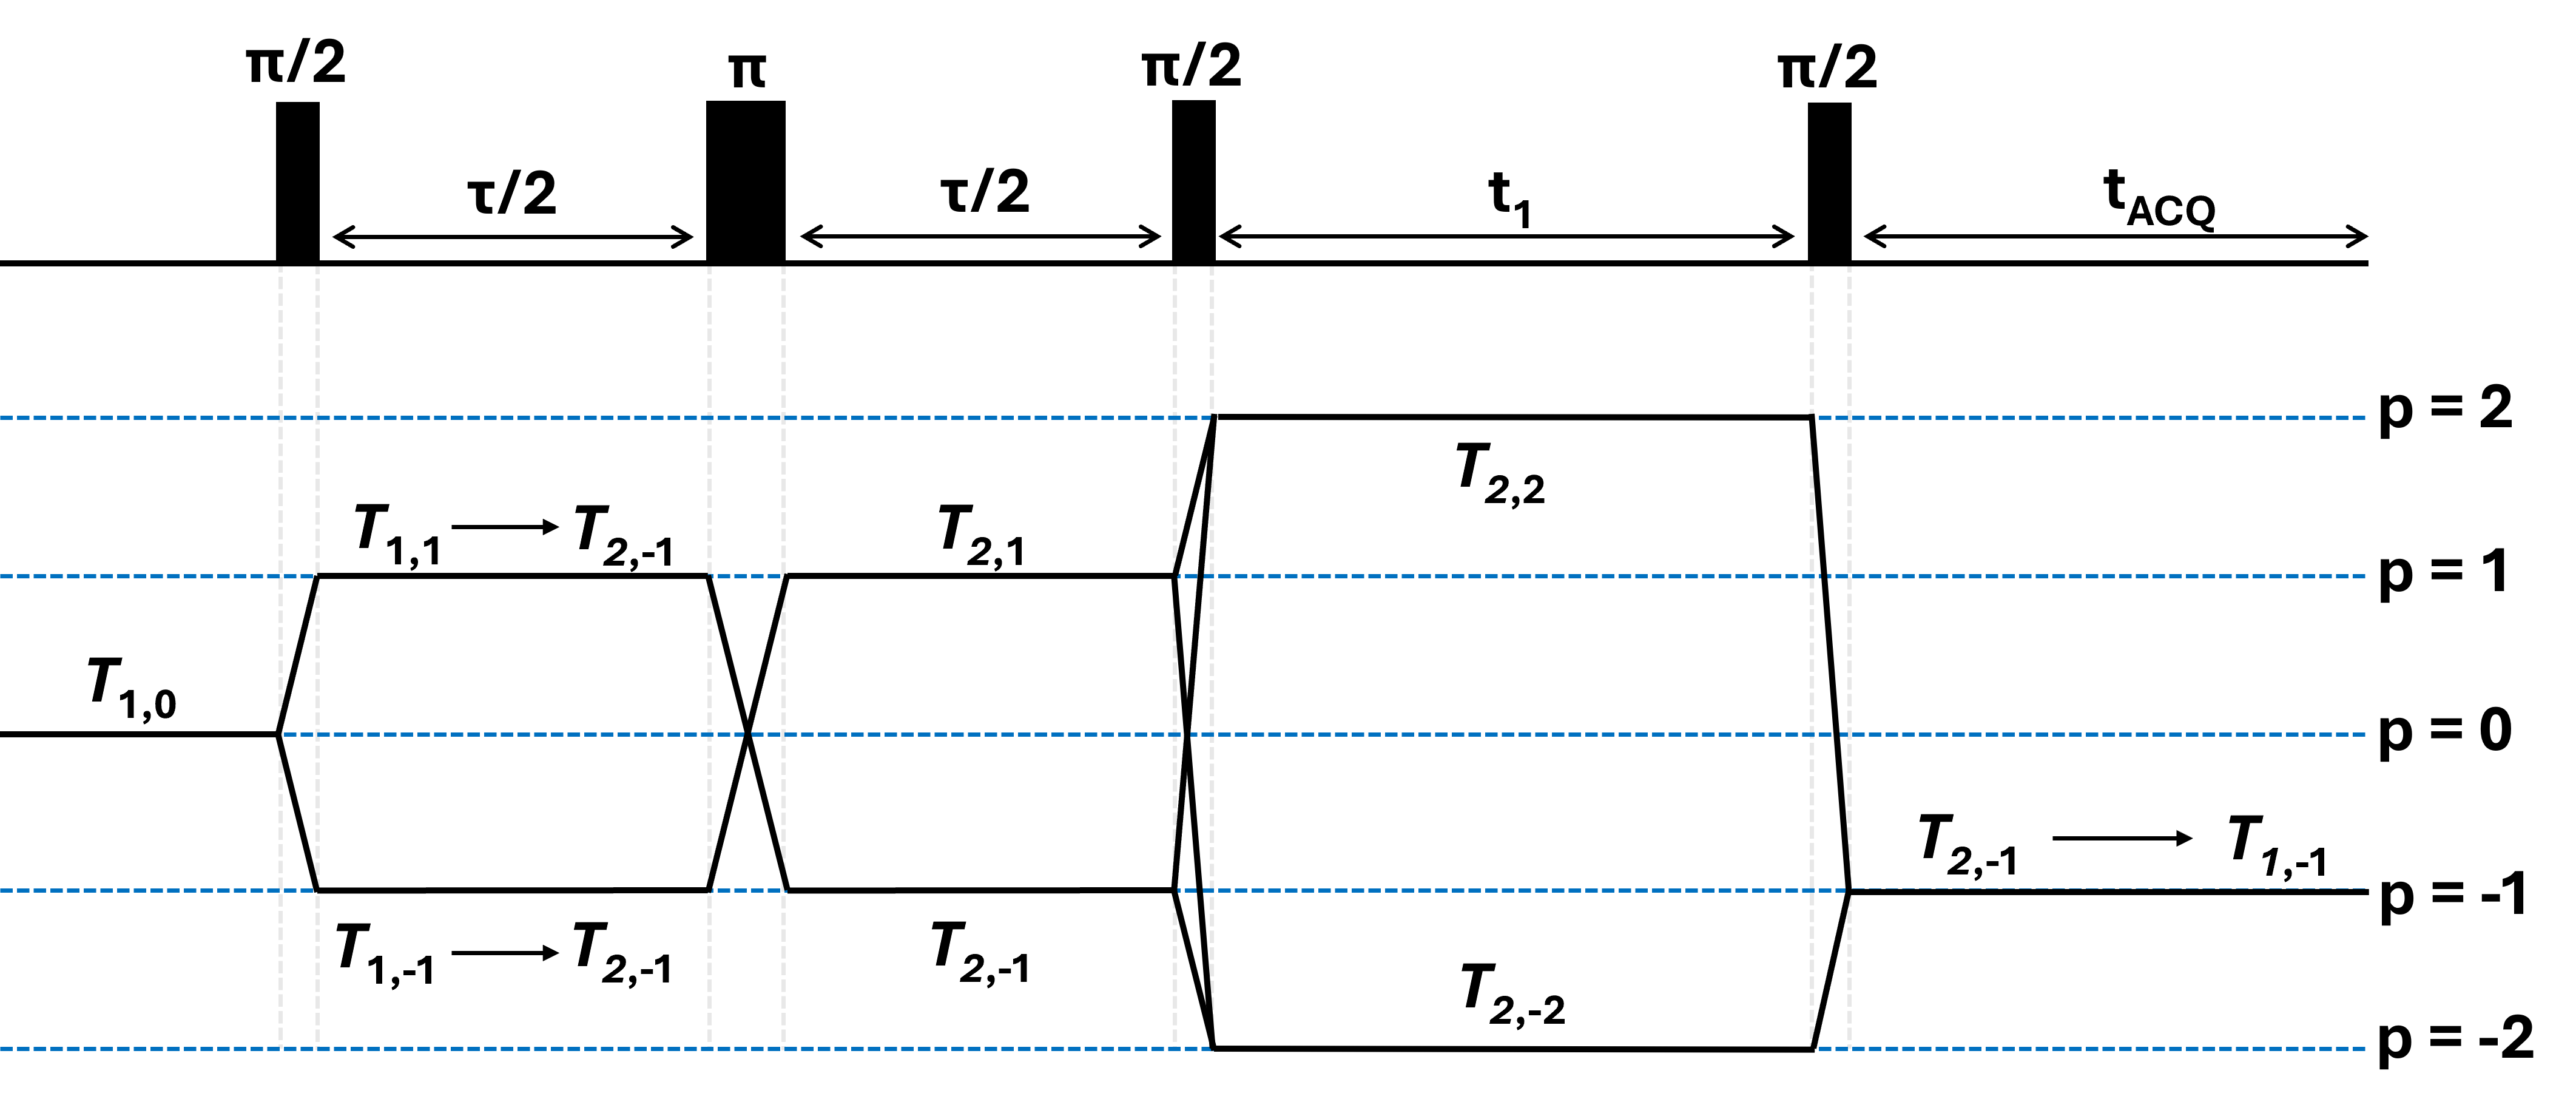
\includegraphics[width=1\textwidth]{Figures/Quad/DQF_Coherence.png}
    \caption{\textit{The coherence pathway and the RF pulse sequence during a \ac{DQF} acquisition. Noting that the tensor $T_{l,p}$ includes information on the rank ($l$) and on the coherence ($p$), which is indicated on the right side. The phase cycling of the last pulse ($\phi$) is x, y, -x, -y and the phase of the receive ($\theta$) is x, -y, -x, y.}}
    \label{fig:Quad:Coherence}
\end{figure}

A pulse sequence that can be used to suppress the single quantum coherence and obtain the double quantum coherence is shown in Fig. \ref{fig:Quad:Coherence} \cite{Sharf1995DetectionNMR-Spectroscopy}, where the pulse angles and the wait times are shown below. It is important that the correct phase cycling is used \cite{Bodenhausen1984SelectionExperiments}, the following transmit phase cycling for the last pulse is $x,\:y,\:-x,\:-y$ and the following receive phase is $x,\:-y,\:-x,\:y$. 

\begin{equation}
    \pi/2-\tau/2-\pi-\tau/2-\pi/2-t_1-\pi/2-t_2 \textrm{ (Acquisition)}
    \label{eqn:Quad:Pulse}
\end{equation}

The phase cycling suppresses the single quantum coherences and preserves the double quantum coherences togethe,r so that the signal is detectable. The obtained FID appears as two anti-phase Lorentzian lineshapes separated by the \ac{RQC}. If this separation is small the presence of two resonances can be difficult to identify as the curves overlap. The amplitude of the \ac{DQF} FID follows a damped sinusoid of the form. 

\begin{equation}
    A\sin(2\pi\nu_q\tau)\exp(-2\tau/T_2)
    \label{eqn:Quad:Amplitude}
\end{equation}

Where $T_2$ is the transverse relaxation time, $A$ is an amplitude coefficient, $\nu_q$ is the splitting frequency and $\tau$ is known as the creation time and is the time between the first two $\pi/2$ pulses. An example \ac{DQF} spectra with corresponding fitting can be seen in Fig. \ref{fig:Quad:Ex_DQF}. This form assumes perfect application of the flip angles shown in Fig. \ref{fig:Quad:Coherence} and that the signal is on-resonance. The coherence transfer pathway with the changing tensor terms can be seen in Figure \ref{fig:Quad:Coherence}.

\begin{figure}
    \centering
    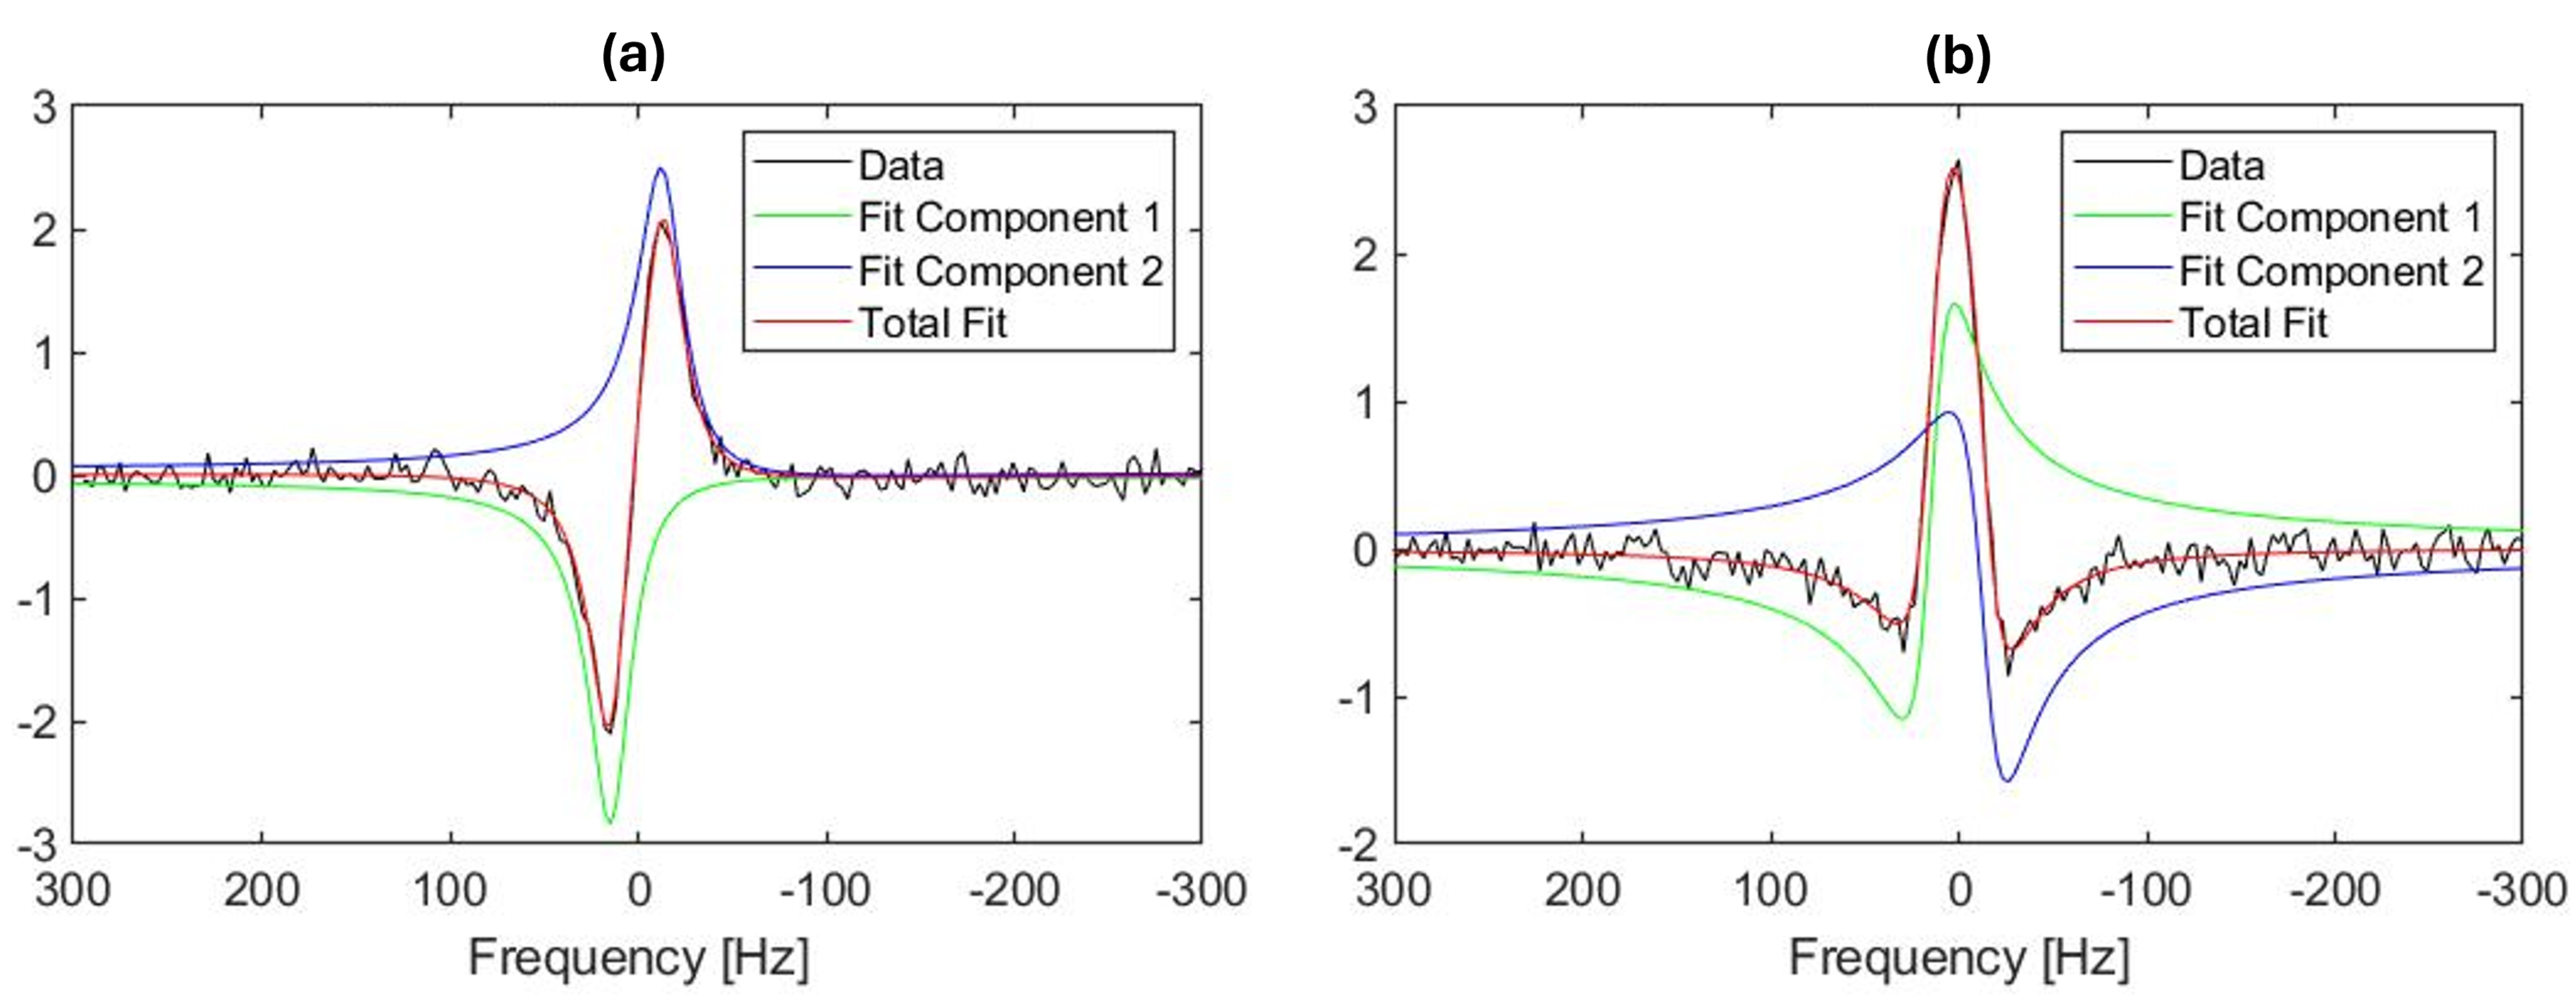
\includegraphics[width=1\textwidth]{Figures/Quad/Example_DQF.png}
    \caption{\textit{\ac{DQF} spectrum from an axial 2 cm slice of the lower leg, acquired with $\tau$ = 6.5 ms. The plots show the fitting of the two independent Lorentzians to the anti-phase \ac{DQF} doublet. The imaginary part of the spectrum (absorption) is shown in (a), the real part (dispersion) is shown in (b). The fitting produces a value for the splitting of $\nu_q$ = 27.7 Hz, and mean $T_2^*$ = 11.3 ms.}}
    \label{fig:Quad:Ex_DQF}
\end{figure}

\section{Scanning}

Measurements for this work was obtained in two separate investigations that both used the ingestion of \ac{D$_2$O} to increase the $^2$H concentration. The initial investigation was setup to look at the spread of $^2$H enrichment in skeletal muscle (see Chapter \ref{Chap:D2O}), however quadrupolar splitting was observed across the calf (most notably in the tibialis anterior muscle). This was used as motivation to investigate the effect of quadrupolar splitting in skeletal muscle, quickly in the first investigation and more seriously in the second investigation. The first investigation was used to formulate the second study and improve the parameters chosen and to improve the aims. Loading routines were implemented in each investigation and both took place at different times. Due to the use of different loading routines the $^2$H abundance were different in different objects and experiments, but the exact \ac{SNR} was not important for either investigations as long as it was possible to obtain data in a reasonable time frame. The loading routine for the first investigation was the same as was used in Chapter \ref{Chap:D2O}, and the loading routine for the second investigation was the same as in Chapter \ref{Chap:Lipid}. Here only results from the second investigation is shown.
% Each part of the first investigation had a different number of participants, while the second investigation had three participants for each part (two of whom also took part in the previous investigation). 

All data was acquired using a Philips 3T Achieva scanner. All $^1$H anatomical scans were performed using the built-in body coil using a 3D \ac{GE} scan. $^2$H data was obtained using in-house built coils details of which can be found in Section \ref{Chap:Theory:Coils} of Chapter \ref{Chap:Theory}. 

% \subsection{Study One}
% \subsubsection{Quadrupolar Splitting}
% \label{Chap:Quad:1:Split}

% After the initial \ac{D$_2$O} loading period was completed and the participants $^2$H enrichment had reached a steady state level. The left calves of two participants (A and B) were scanned using the in-house built $^2$H saddle coil. 3D \ac{CSI} were obtained with 10 mm isotropic voxels, NSA = 2, samples = 256, \ac{TE} = 6.2 ms, \ac{TR} = 500 ms, \ac{BW} = 750 Hz, FOV = 120x120x60 mm$^3$, the \ac{CSI} data was originally acquired to investigate the overall spread of $^2$H enrichment in skeletal muscle (see Chapter \ref{Chap:D2O}). However quadrupolar splitting was observed across the calf (most notably in the tibialis anterior muscle). This was used as motivation to investigate the effect of quadrupolar splitting in skeletal muscle.
% The participants were therefore scanned again using the in-house built Helmholtz coil designed to scan the forearm. The left forearms of A and B were scanned as this allowed us to easily bend the arm in the coil at different angles with respect to the $B_0$ field of the magnet, which allows us to change $\theta$ in equation \ref{eqn:Quad:Angle}. A $^2$H 3D \ac{CSI} with 10x10x15 mm$^3$ voxels, NSA = 2, 256 samples, \ac{TE} = 6.4 ms, \ac{TR} = 363 ms, \ac{BW} = 750 Hz and \ac{FOV} = 120x120x60 mm$^3$ is acquired for a range of different arm angles was acquired. During scanning, for each angle, participants were lay in a prone position with their left arm above their head. A 'straight' arm represented  0$^{\circ}$ angle respect to the $B_0$ field, participant A was then scanned with angles of 0, 10, 20, 30 and 40$^{\circ}$ in one visit and 50, 60, 70, 80 and 90$^{\circ}$ in a second visit. Participant B was scanned with angles 0, 85, 30, 15, 45, 60, 75 and -10$^{\circ}$ in a single visit. 
% The 3D \ac{CSI} spectra for the forearm was analysed using MATLAB and started with zero-order phase correction and masked based on the maximum value from the spectra of a specific voxel being larger than 20\% of the maximum value of all spectra. Each voxel within the mask was then fit to two complex Lorentzian curves with equal amplitudes, phases and linewidths where the frequency splitting between the two peaks is determined from fitting. The spectra is also fit to three complex Lorentzian curves where the two 'outer' peaks have equal equal amplitudes, phases and linewidths similar to before except now there is a third central peak with different amplitude, phase and linewidth to the other peaks the frequency splitting is now the frequency difference between the 'outer' two peaks only. The fitting is performed by minimising the sum of the squared difference between the proposed fit and the phase-corrected signal, this was done using in-built MATLAB function fmincon. The best fit is determined by comparing the final minimised value returned from fitting, whichever combination of Lorentzian curves gave the lowest value is kept and outputted for that voxel. The frequency splittings are then averaged over the masked region to give a single frequency splitting. This process was repeated for each angle, with the angle values being obtained from the angulation of the imaging/spectroscpy \ac{FOV}. All the splitting's were then fit to equation \ref{eqn:Quad:Angle}, where the total \ac{RQC} is determined. This was repeated for participants A and B.

% \subsubsection{Double Quantum Filtering}
% \label{Chap:Quad:1:DQF}

% $^2$H spectroscopy and \ac{CSI} were performed on lower legs and forearms in four healthy human participants (A,B,C and D). $^2$H spectra were acquired from a 2 cm axial slice of the calf or forearm, by using hard pulses in combination with outer-volume saturation. \ac{DQF} spectra were created by using the sequence in Figure \ref{fig:Quad:Coherence}, which produces an anti-phase spectrum whereby the quadrupolar doublet peaks acquire a relative phase of 180$\circ$ (see Figure \ref{fig:Quad:Ex_DQF}). This relative phase means that the signal vanishes for any components if their splitting frequency is small. \ac{DQF} spectra are phased to produce a symmetric line-shape (labelled as dispersion spectra in anti-phase in Figure \ref{fig:Quad:Ex_DQF}).  
% \ac{DQF} spectra were acquired for various values of $\tau$, and \ac{TR} = 1000 ms, \ac{TE} = 0.58 ms, \ac{BW} = 3000 Hz, samples = 1024. The number of averages varied, depending on available signal, between 28 and 128. \ac{FID}s were processed using Matlab scripts and spectra were fit to a maximum of three independent Lorentzian line shapes.
% $^2$H 2D \ac{CSI} data were also acquired from a single 2 cm axial slice, again using outer-volume suppression. 2D \ac{CSI} data were acquired for the usual pulse-acquire sequence, and using the anti-phase \ac{DQF} sequence with $\tau$ = 6.5 ms. The voxel volume was 10x10 mm$^2$, \ac{TR} = 378 ms, \ac{TE} = 3.9 ms, samples = 256 and \ac{BW} = 750 Hz. For the \ac{DQF} \ac{CSI}, 16 averages were acquired, whereas only 4 were needed for the pulse-acquire \ac{CSI}.

% \subsection{Study Two}
% \subsubsection{Quadrupolar Splitting}

\subsection{Quadrupolar Splitting}

After the initial \ac{D$_2$O} loading period was completed and the participants $^2$H enrichment had reached a steady state level. $^2$H 3D \ac{CSI} data were acquired again with 10x10x10 mm$^3$ voxels, \ac{FOV} = 120x120x50 mm$^3$, \ac{TR} =500 ms, \ac{TE} = 6.2 ms, \ac{BW} = 750 Hz, samples = 256 and NSA = 2 in the forearm of three healthy human participants using an in-house built Helmholtz coil. Images were acquired in each subject with the forearm at 10 different angles ($\approx$0 – 90$^\circ$) to the field. 
% The protocol here was similar to what followed in the above section (chapter \ref{Chap:Quad:1:Split}). 

In order to ensure that the forearm was always in the centre of the field, that a large enough range of angles were covered and that each participant was as comfortable as they could be. Each participant was removed from the scanner in between acquisition of data at each angle, which is why commonly scanning ran over two days. The protocol for each angle included  acquisition of a $^1$H scout scan and \ac{GE} anatomical images, two bulk spectra and finally a 3D \ac{CSI}. 
% For angles larger than 45$^\circ$ the data had to be acquired sagittally as oppose to transverse.

Whilst this study was similar what was performed in the first investigation, one of the major differences is in the analysis routine. As the arm is a large muscle it can be difficult to estimate the angle relative to the magnetic field. A paper compass attached to the top of the coil helped to orient the arm in the scanner, but in the previous work the angle was automated when planning the acquisition on the $^1$H scout scan. Here the angle of the arm was calculated by measuring the angle of the ulna bone using the Mango software (https://mangoviewer.com/download.html), which was found to be different from the angle estimated from the compass.

Zero-order phase correction was applied to all spectra, as well as de-noising through a Tucker decomposition \cite{Bader2007EfficientTensors} with a compression core matrix of [64,6,6,3] (spectral, followed by three spatial dimensions). A binarised mask with the same spatial resolution as the \ac{CSI} data is then constructed, following thresholding of 35\% of the maximum spectral signal (the mask was then filled using imfill). The OXSA-AMARES \cite{Purvis2017OXSA:MATLAB} toolbox in Matlab was then used to fit three Lorentzian peaks to each masked voxel, centre peak with an outside doublet due to quadrupolar splitting (each peak in the doublet has the same linewidth and amplitude, all peaks are fit with the same phase). The initial estimate of the seperation of the doublet varied depending on the angle of the arm in the scanner. The separation of the doublet was converted from ppm to Hz and then the values, along with the arm angle, was fitted to Eq. \ref{eqn:Quad:Angle}.

% \subsubsection{Double Quantum Filtering}
\subsection{Double Quantum Filtering}

\ac{DQF} $^2$H non-localised spectra were acquired again from a 2-cm axial slice of the forearm, using hard pulses in combination with outer-volume saturation in three healthy human participants. Spectra were obtained via an anti-phase \ac{DQF} sequence \cite{Sharf1995DetectionNMR-Spectroscopy} whereby the quadrupole-doublet peaks acquire a relative phase of 180$^\circ$. \ac{DQF} spectra were acquired for a range of values of the creation time, $1\leq\tau\leq36$ ms (a larger range and more values compared to investigation one), with \ac{TR} = 1000 ms, \ac{TE} = 0.58 ms, \ac{BW} = 3000 Hz, samples = 1024 and NSA = 56.

$^2$H 2D \ac{CSI} data were also acquired from a single slice, using outer-volume suppression and using the anti-phase \ac{DQF} sequence (\ac{DQF}-\ac{CSI}) with $\tau$ = 5 ms in both the lower leg and forearm. Each voxel for the \ac{CSI} was 10x10 mm$^2$ in-plane, \ac{TR} = 1000 ms, \ac{TE} = 2 ms, samples = 256, bandwidth = 750 Hz, NSA = 8 with a slice thickness of 30 cm. $^1$H scout and 3D \ac{GE} (2 mm isotropic voxels, \ac{TR} = 20 ms, \ac{TE}, 2.1 ms, \ac{FOV} = 128x128x192 mm$^3$, NSA = 1) anatomical images were also obtained, along with $^2$H 2D \ac{SQF}-\ac{CSI} data with the same scan parameters as the $^2$H 2D \ac{DQF}-\ac{CSI} scans. The forearm measurements were then repeated for a range of angles to the $B_0$ magnetic field, the angles of the coil were 0$^\circ$, 30$^\circ$, 60$^\circ$ and 90$^\circ$. 

The non-localised spectra were apodised using a 5 Hz exponential line-broadening filter to increase \ac{SNR}, whilst the \ac{CSI} data was de-noised using a Tucker decomposition \cite{Bader2007EfficientTensors} with a core matrix of [32, 6, 6, 2] (time, two spatial and angular dimensions respectively) to increase \ac{SNR}. All \ac{DQF} spectra were fit using the OXSA-AMARES \cite{Purvis2017OXSA:MATLAB} toolbox in MATLAB, using two Lorentzian peaks with 180$^\circ$ phase difference, equal linewidths and equal amplitudes determined in the prior knowledge. Automatic zeroth-order phase correction was also applied to each spectra. Then four similar voxels were averaged across each subject and all angles and the spectra compared.

% \section{Results}
% \subsection{Study 1}
% \begin{figure}
%     \centering
%     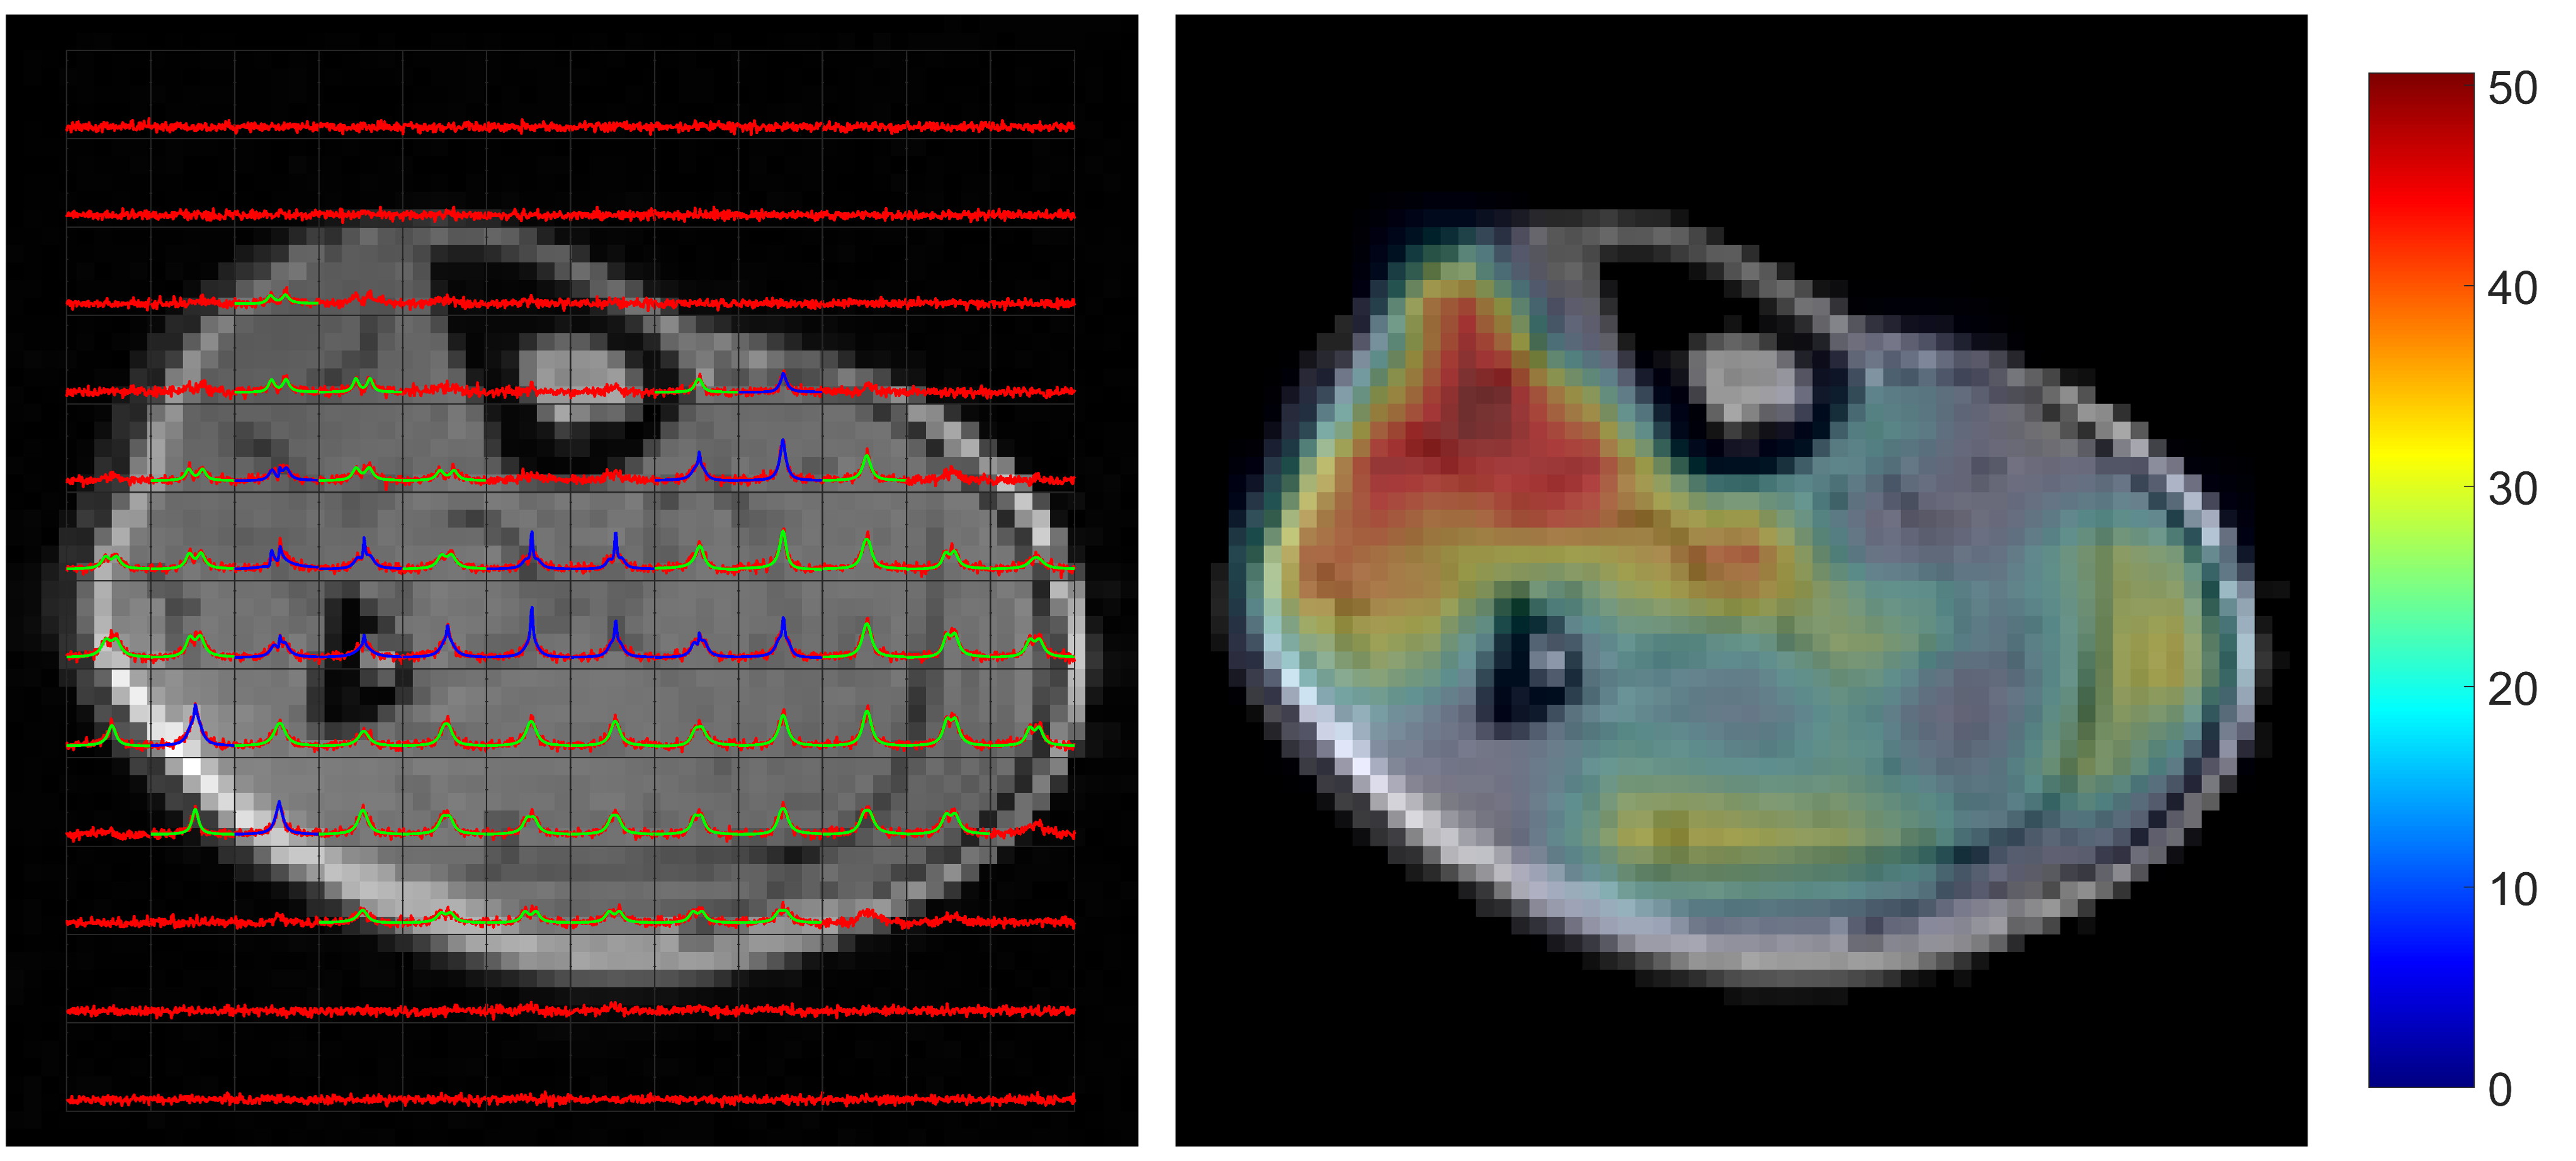
\includegraphics[width=1\textwidth]{Figures/Quad/Calf_A.png}
%     \caption{\textit{Left: \ac{CSI} spectra (red) overlayed onto a $^1$H \ac{GE} image from participant A's left calf of a single slice, with fits of two Lorentzian peaks (green) and three Lorentzian peaks (blue). Right: Interpolated map of quadrupolar frequency splitting's overlayed onto the same $^1$H \ac{GE} image from participant A's left calf.}}
%     \label{fig:Quad:Calf_A}
% \end{figure}
% \begin{figure}
%     \centering
%     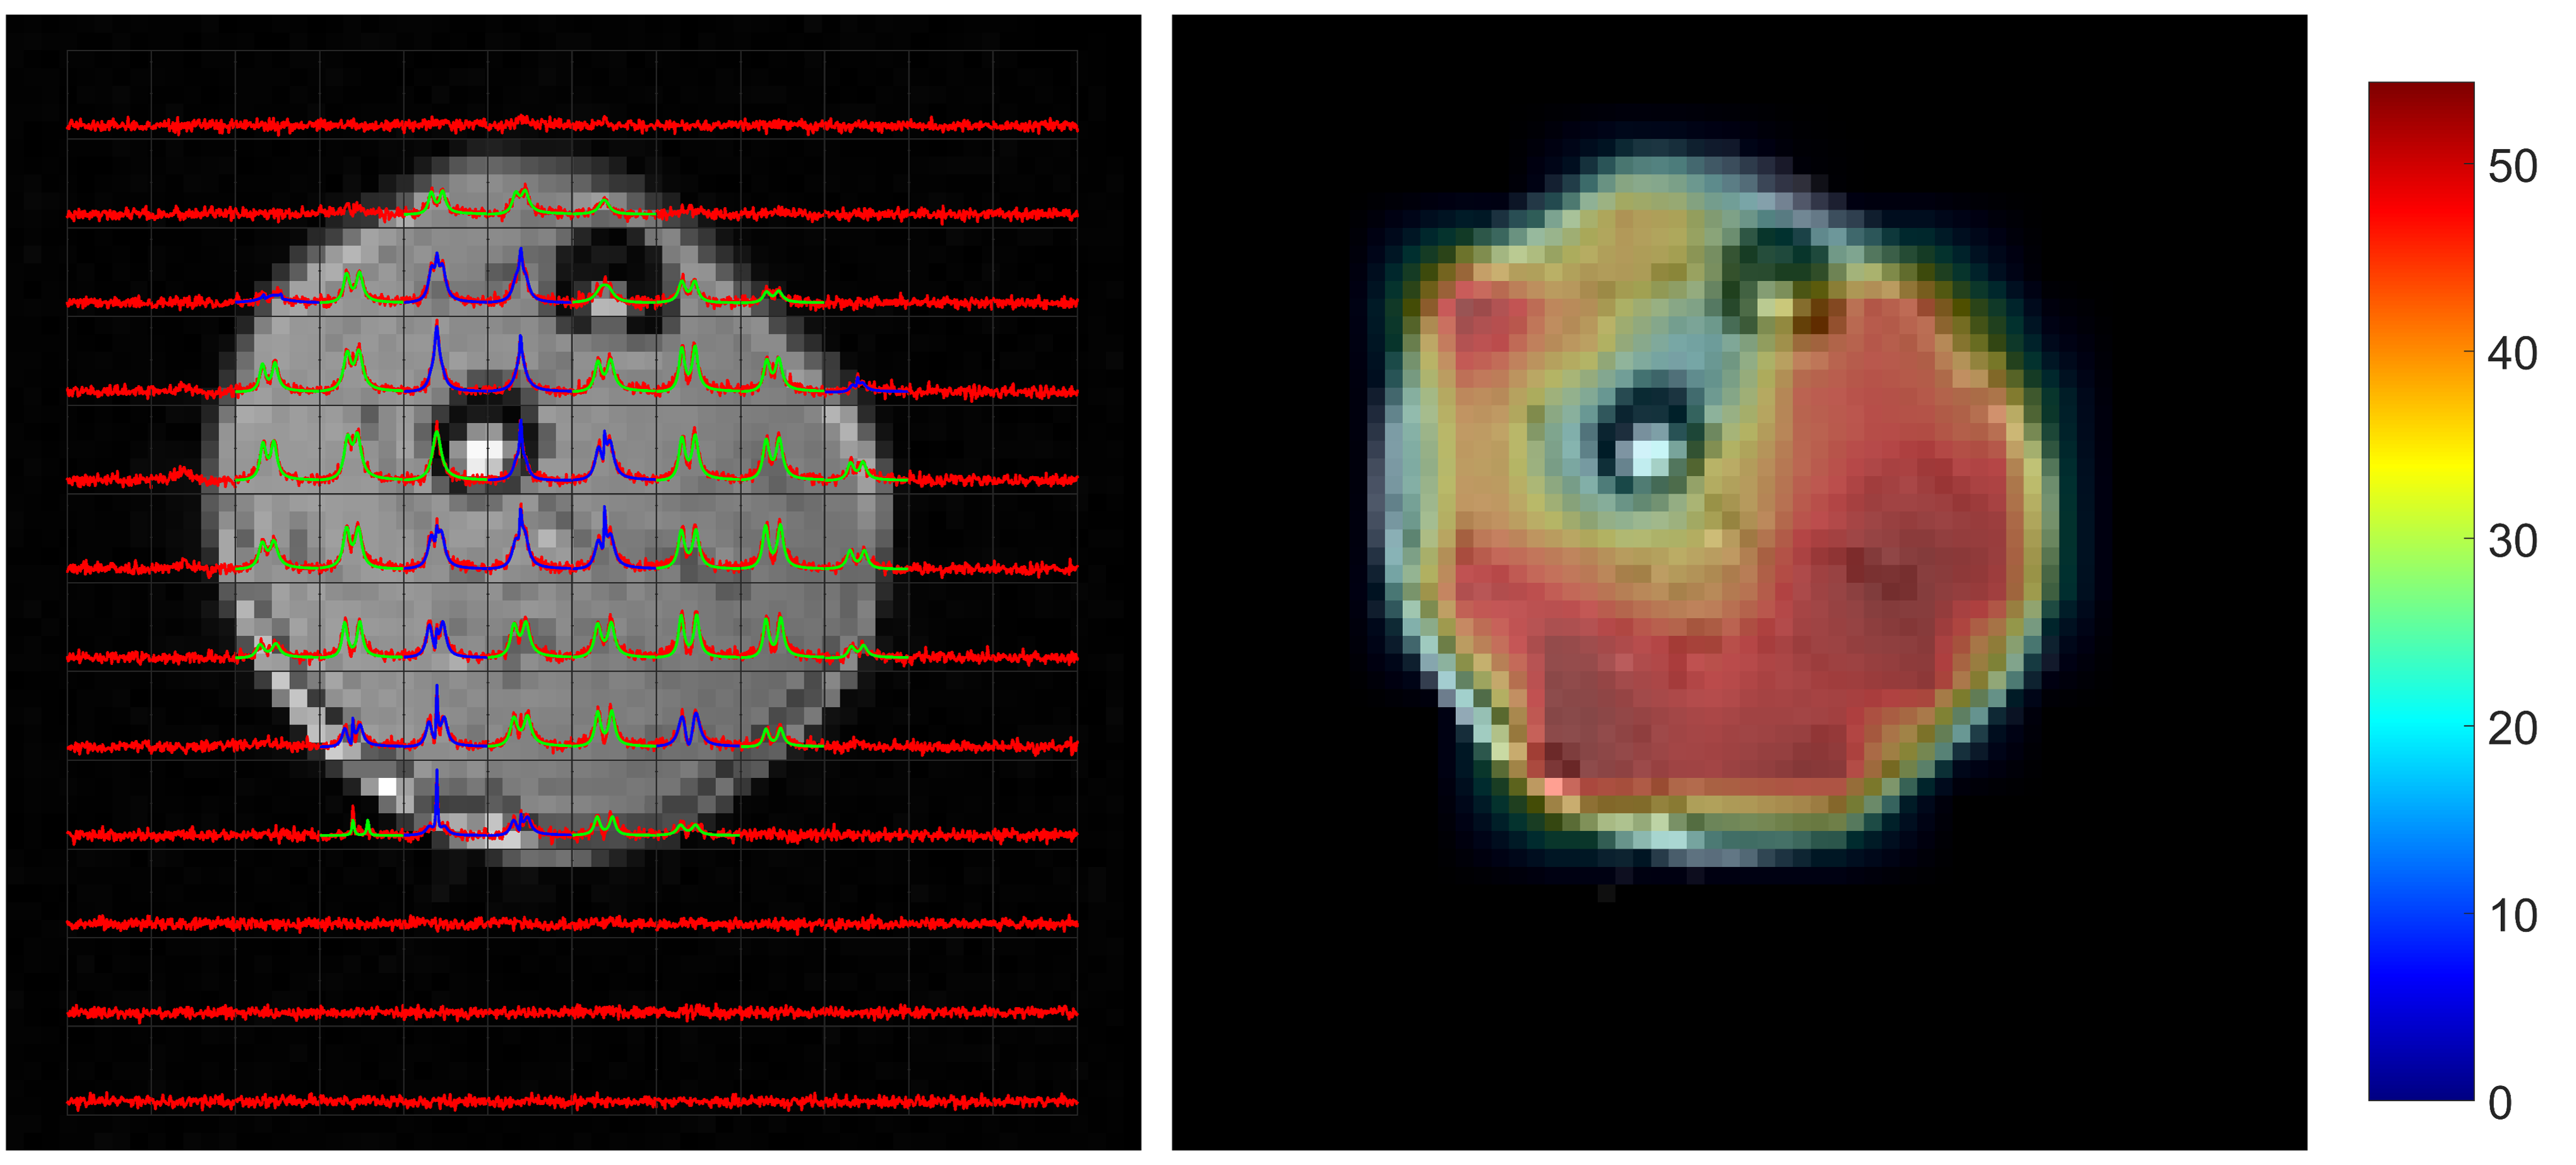
\includegraphics[width=1\textwidth]{Figures/Quad/Arm_A.png}
%     \caption{\textit{Left: \ac{CSI} spectra (red) overlayed onto a $^1$H \ac{GE} image from participant A's left arm at an angle of 0$^\circ$ to the $B_0$ field of a single slice, with fits of two Lorentzian peaks (green) and three Lorentzian peaks (blue). Right: Interpolated map of quadrupolar frequency splitting's overlayed onto the same $^1$H GE image from participant A's left arm.}}
%     \label{fig:Quad:Arm_A}
% \end{figure}
% Figures \ref{fig:Quad:Calf_A} and \ref{fig:Quad:Arm_A} show spectra acquired from $^2$H \ac{CSI} data acquired in the lower leg and forearm (respectively). Though some of the spectra are analysed are analysed differently to others, being fit with two Lorentzian peaks (green) as opposed to three (blue). On the right side of each Figure the overlayed frequency splittings in Hz, after it has been interpolated to the same resolution as the $^1$H anatomical image. There is obvious in-homogeneity in the frequency splitting in Figure \ref{fig:Quad:Calf_A} with increased splitting covering the \ac{TA} muscle and slightly the Gastrocnemius muscle. The frequency splitting is more homogeneous in the arm with the only notable decrease being present over the radial and ulna bones.
% \begin{figure}
%     \centering
%     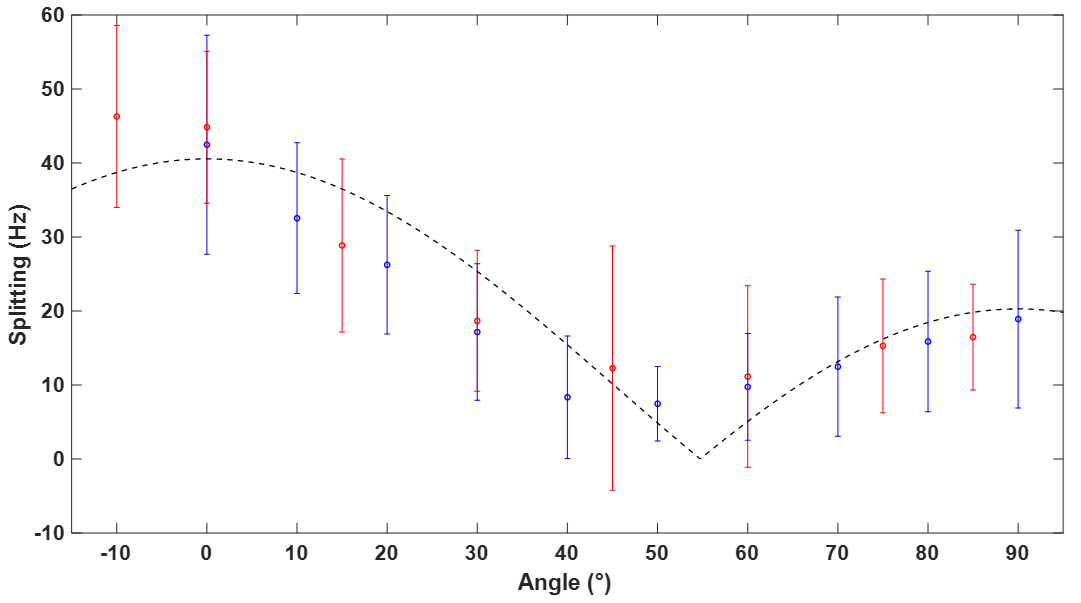
\includegraphics[width=1\textwidth]{Figures/Quad/Split_Angle_1.png}
%     \caption{\textit{Graph Showing the variation of averaged quadrupolar frequency splittings of the arm against the angle to the $B_0$ field they were positioned at, for partcipant A (blue) and B (red). Along with the fit (dotted black) of both participant's data to equation \ref{eqn:Quad:Angle}, the splitting magnitude of this fit is 38 $\pm$ 2 Hz.}}
%     \label{fig:Quad:Split_Angle_1}
% \end{figure}
% Both the lower leg and forearms in Figures \ref{fig:Quad:Calf_A} and \ref{fig:Quad:Arm_A} are aligned to the external magnetic field $B_0$. The forearm is then rotated over a range of angles (-10$^\circ$ to 90$^\circ$) with the previous methodology repeated averaging over the full \ac{ROI} obtaining a single value for the splitting and fitting to equation \ref{eqn:Quad:Angle}, which can be seen as a black dotted line in Figure \ref{fig:Quad:Split_Angle_1}. The angle used here is the angle of the imaging/scanning \ac{FOV}. From this fitting a magnitude value for the splitting value, 38 $\pm$ 2 Hz, is found. From equation \ref{eqn:Quad:Angle} a minimum is found at the magic angle 54.74$^\circ$, a general trend of the splitting decreasing as the angle of the \ac{FOV} is seen here.
% \begin{figure}
%     \centering
%     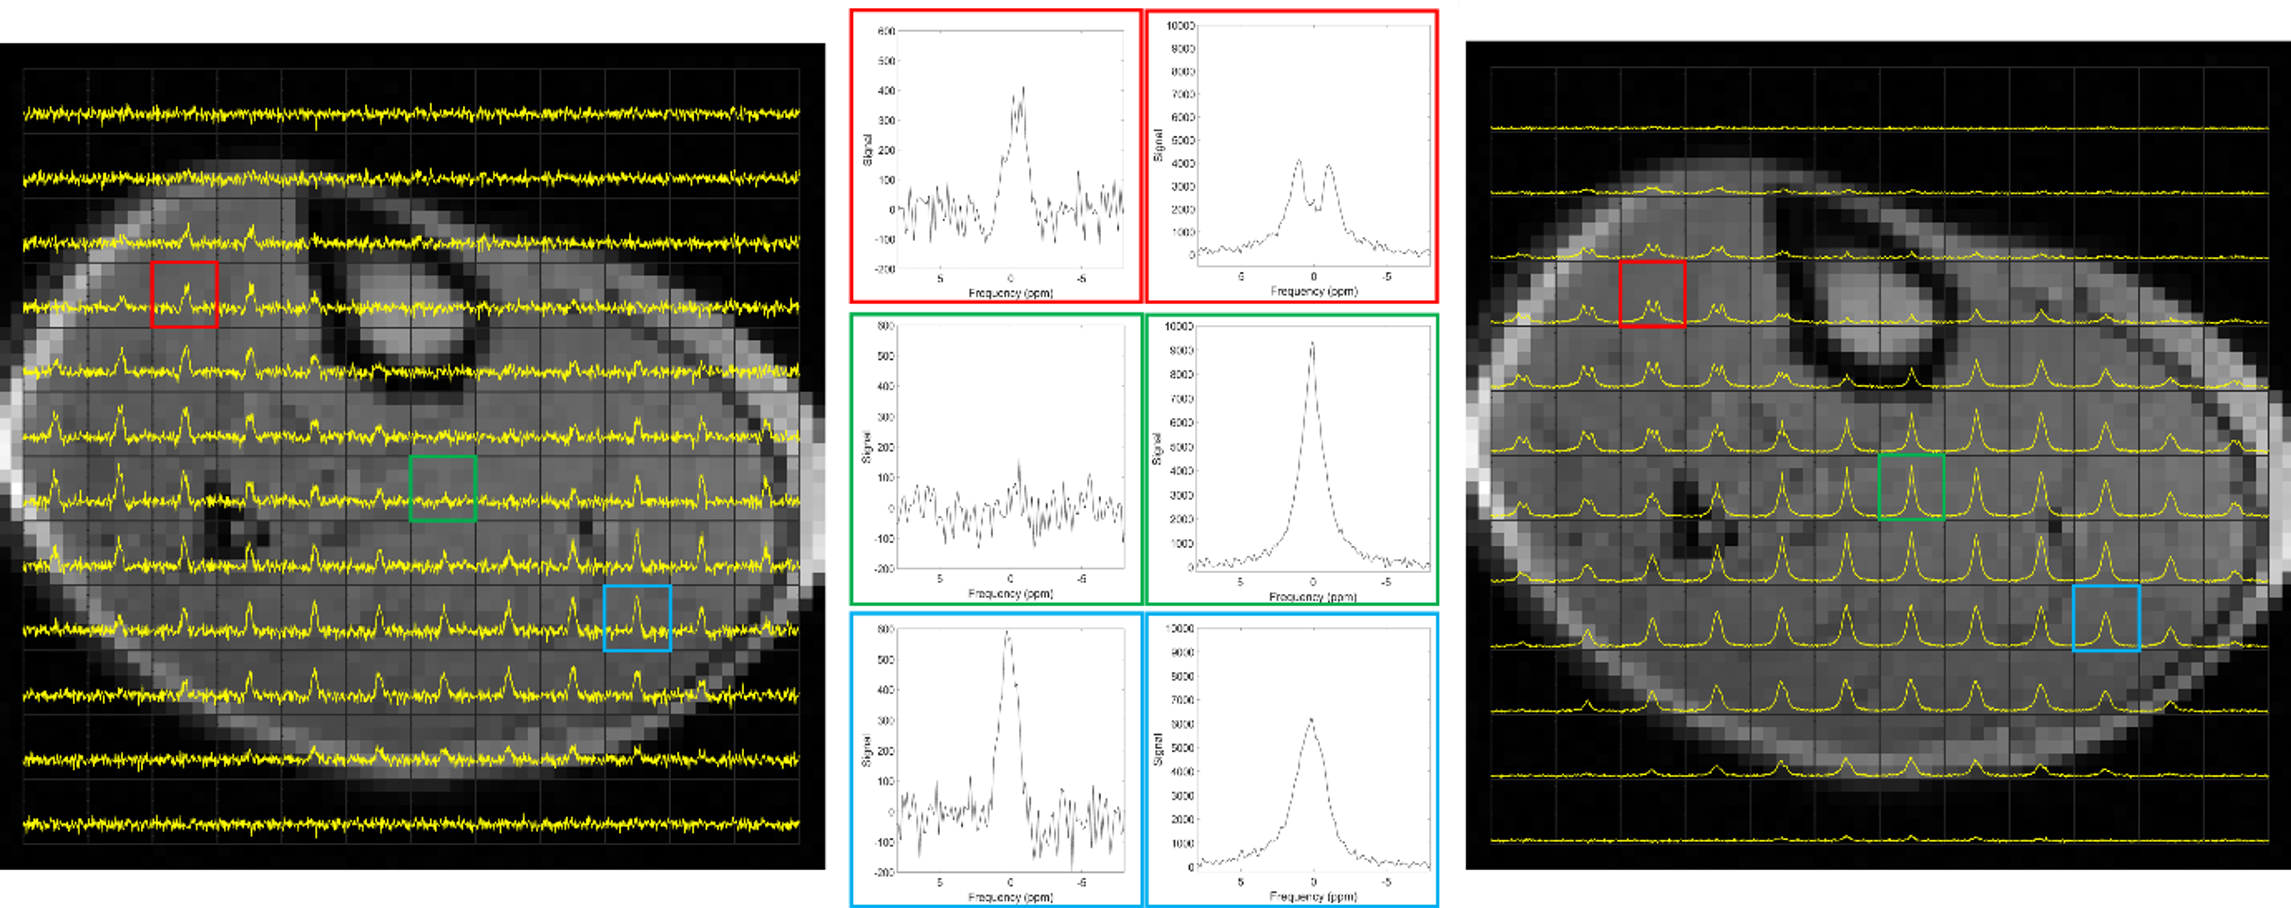
\includegraphics[width=1\textwidth]{Figures/Quad/SQFDQF_CSI_1.png}
%     \caption{\textit{$^2$H \ac{DQF} \ac{CSI} (left) and pulse-acquire \ac{CSI} (right) data obtained from a 2 cm axial slice of the lower leg of the same volunteer with 1cm in-plane resolution. In the centre are spectra from three selected voxels so that a direct comparison can be made of the \ac{DQF} (left) and pulse-acquire (right) spectra from different muscle regions.}}
%     \label{fig:Quad:SQFDQF_1}
% \end{figure}
% Figure \ref{fig:Quad:SQFDQF_1} shows $^2$H \ac{CSI} spectra overlaid on $^1$H \ac{GE} images of the lower leg, for both the \ac{DQF} \ac{CSI} (left) and pulse-acquire \ac{CSI} data (right). Individual \ac{DQF} and \ac{CSI} spectra from three voxels in different muscle groups are also shown in more detail. The red voxel is located in the \ac{TA}, the blue is from the gastrocnemius muscle and the green is from the largest muscle the Soleus. The difference in \ac{SNR} between the two datasets is the key feature between the two scans.
% \begin{figure}
%     \centering
%     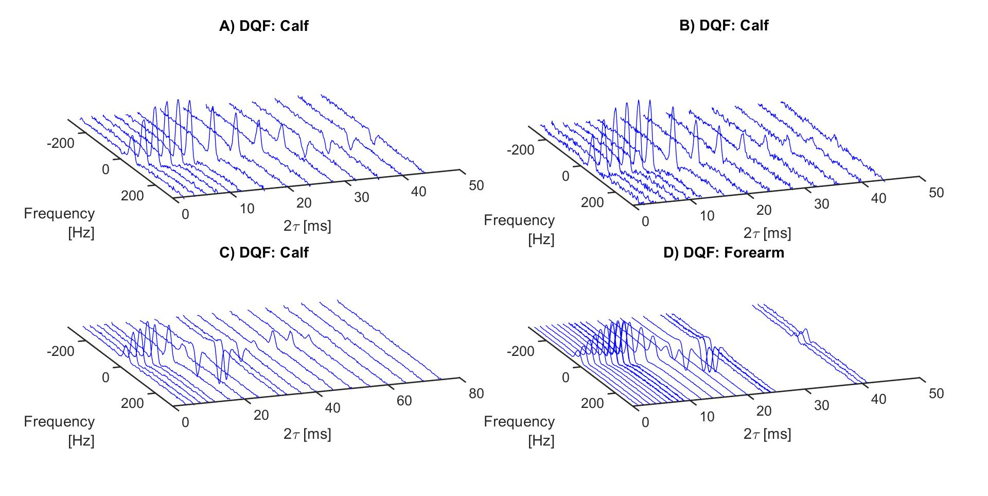
\includegraphics[width=1\textwidth]{Figures/Quad/Bulk_DQF_1.png}
%     \caption{\textit{Deuterium \ac{DQF} spectra acquired from a 2 cm slice of the lower leg (of different volunteers) and forearm with different values of the creation time $\tau$.}}
%     \label{fig:Quad:Bulk_DQF_1}
% \end{figure}
% Figure \ref{fig:Quad:Bulk_DQF_1} shows examples of four, phase-corrected, \ac{DQF} spectral datasets (three lower leg, one forearm) acquired from 2 cm axial slices, acquired with a range of $\tau$ values. The correct phase correction when displaying \ac{DQF} plots as the point at which the amplitude becomes positive is important. The calf measurements appear to evolve much faster compared to the calf, with negative amplitudes even being recorded. Each spectrum was fitted to two independent Lorentzian peaks (as illustrated in Figure \ref{fig:Quad:Ex_DQF}) from which the mean amplitude was plotted as a function of. Examples of these \ac{DQF} plots are shown in Figure \ref{fig:Quad:BuildUp} (two forearms, two lower legs). 
% \begin{figure}
%     \centering
%     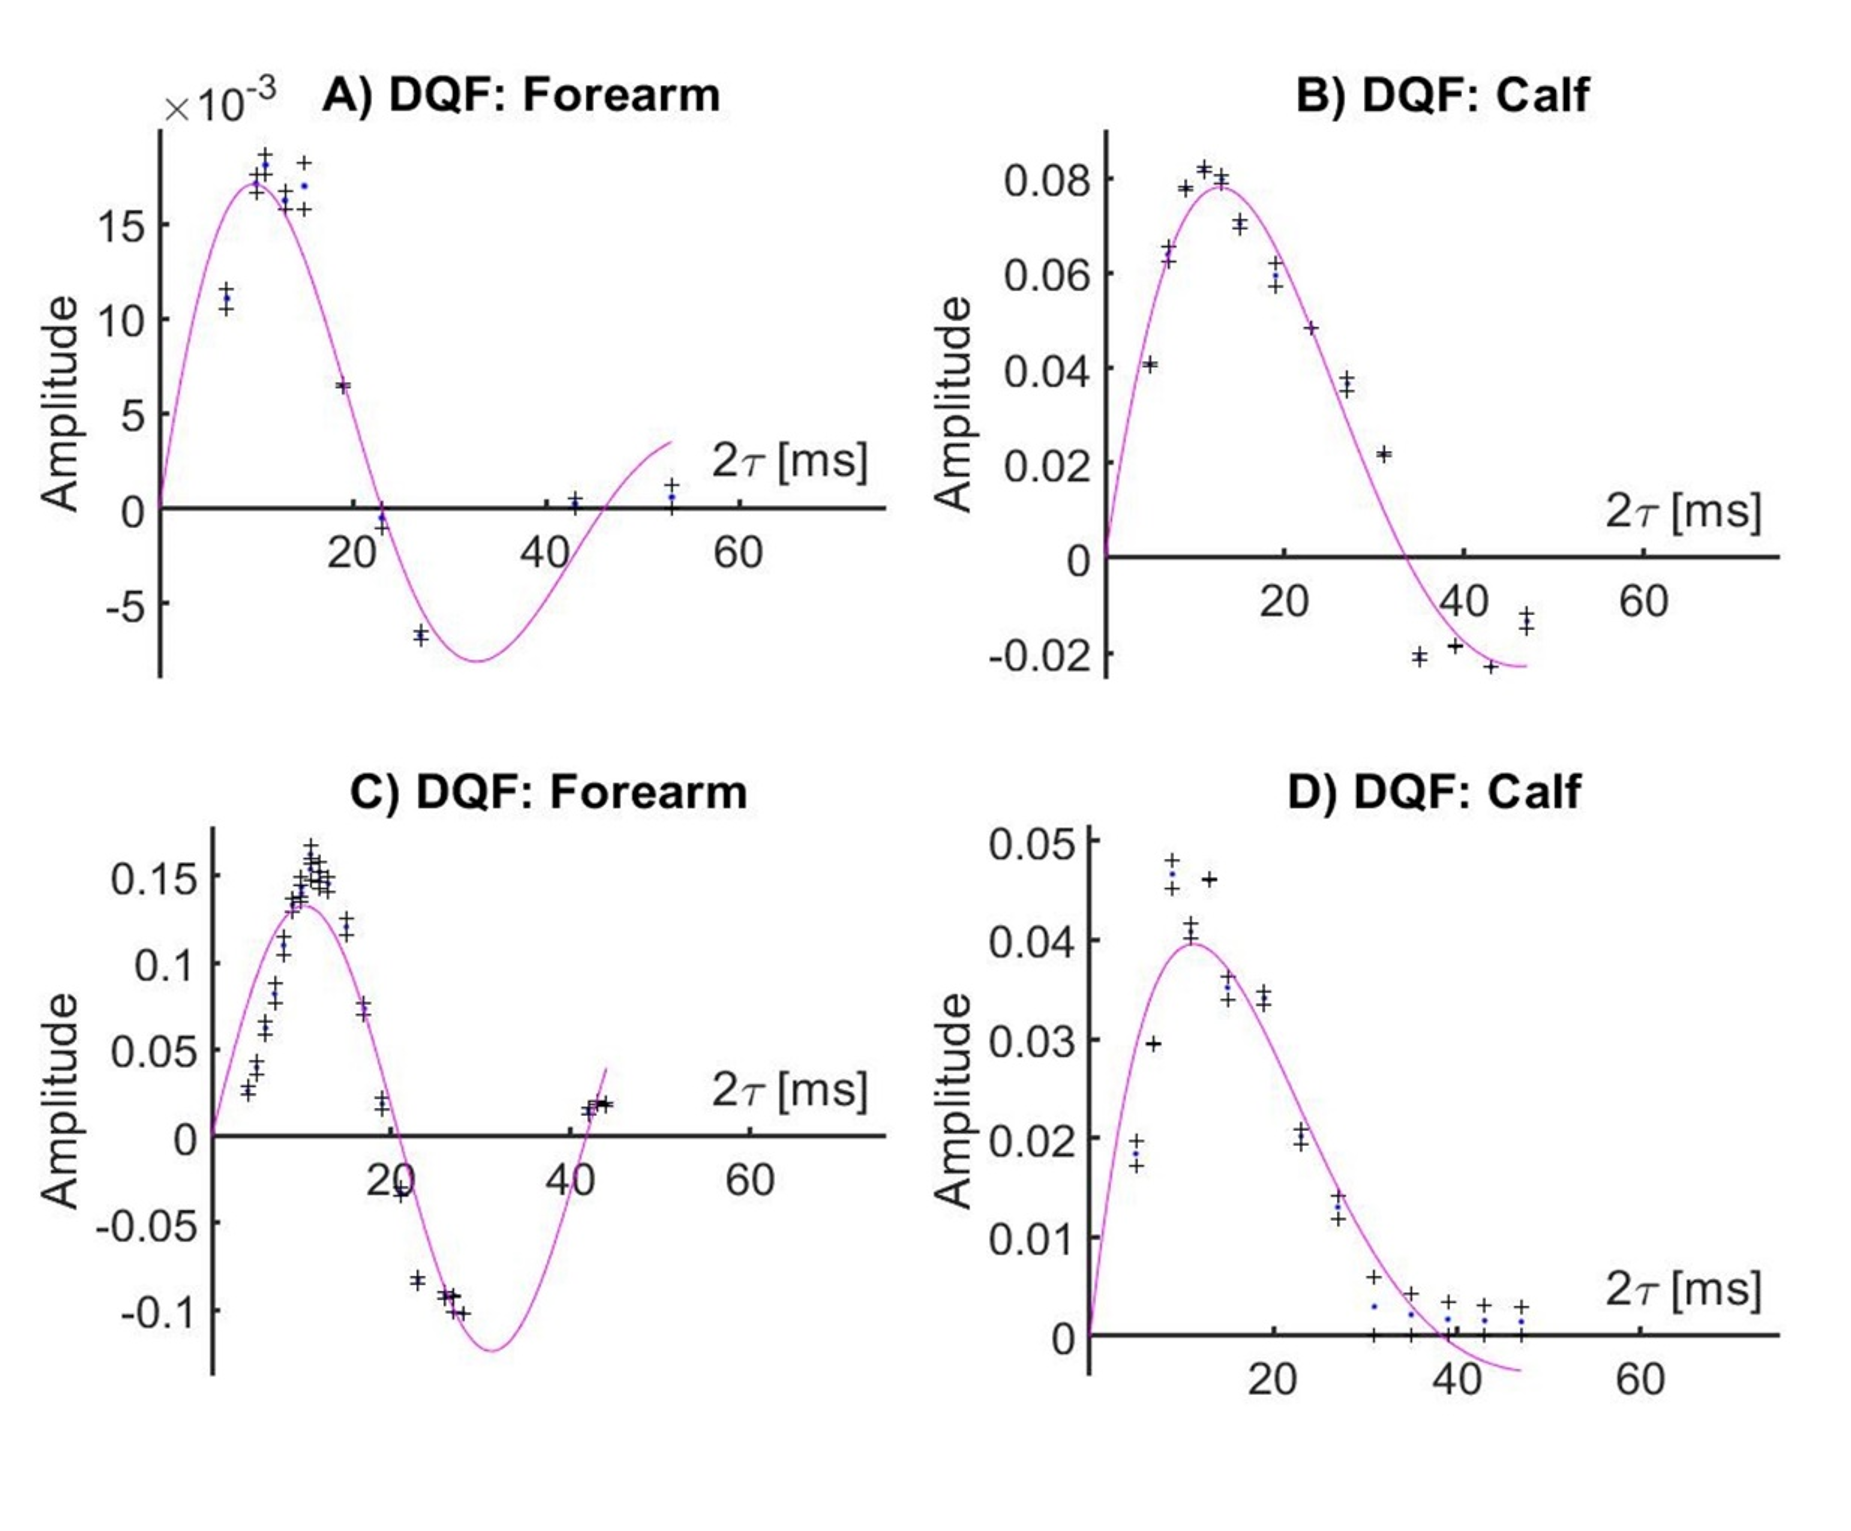
\includegraphics[width=1\textwidth]{Figures/Quad/BuildUp.png}
%     \caption{\textit{\ac{DQF} amplitudes obtained by fitting anti-phase line shapes to spectra obtained from the lower leg and forearm (of different volunteers) as a function of the creation time $\tau$. Continuous magenta lines show fits to the \ac{DQF} amplitude variation with $\tau$ of the form equation \ref{eqn:Quad:Amplitude}. The amplitude term varies across datasets because of the use of different RF coils and the different levels of \ac{D$_2$O} loading in different volunteers.}}
%     \label{fig:Quad:BuildUp}
% \end{figure}
% \subsection{Study Two}

\section{Results}

Figure \ref{fig:Quad:Calf_Arm_CSI} shows single slices from 3D \ac{CSI} acquisitions of the lower leg and forearm, with the limb approximately aligned with the $B_0$-direction. The fitting is performed on a voxel-wise basis and is the same over the whole \ac{ROI} and uses the OXSA-AMARES toolbox \cite{Purvis2017OXSA:MATLAB} implementing prior knowledge, and has been de-noised. The splitting map has not been interpolated here, and can be seen to the follow the general trend in the underlying anatomical image. Doublets can be observed in many voxels, with residual quadrupolar splittings of 20 – 40 Hz. An increase in the \ac{TA} muscle can be seen here with more homogeneity present in the forearm.
% The results here are similar to figures \ref{fig:Quad:Calf_A} and \ref{fig:Quad:Arm_A}. The main differences are that the fitting routine here is the same over the whole \ac{ROI} now (which uses prior knowledge), and de-noising has been applied and the frequency splitting has not been interpolated. The fitting matches the underlying data better here compared to figures \ref{fig:Quad:Calf_A} and \ref{fig:Quad:Arm_A}. Doublets can be observed in many voxels, with residual quadrupolar splittings of 20 – 40 Hz. The same trend over muscle groups as in figures \ref{fig:Quad:Calf_A} and \ref{fig:Quad:Arm_A} with an increase in the \ac{TA} muscle and more homogeneity in the forearm.

\begin{figure}
    \centering
    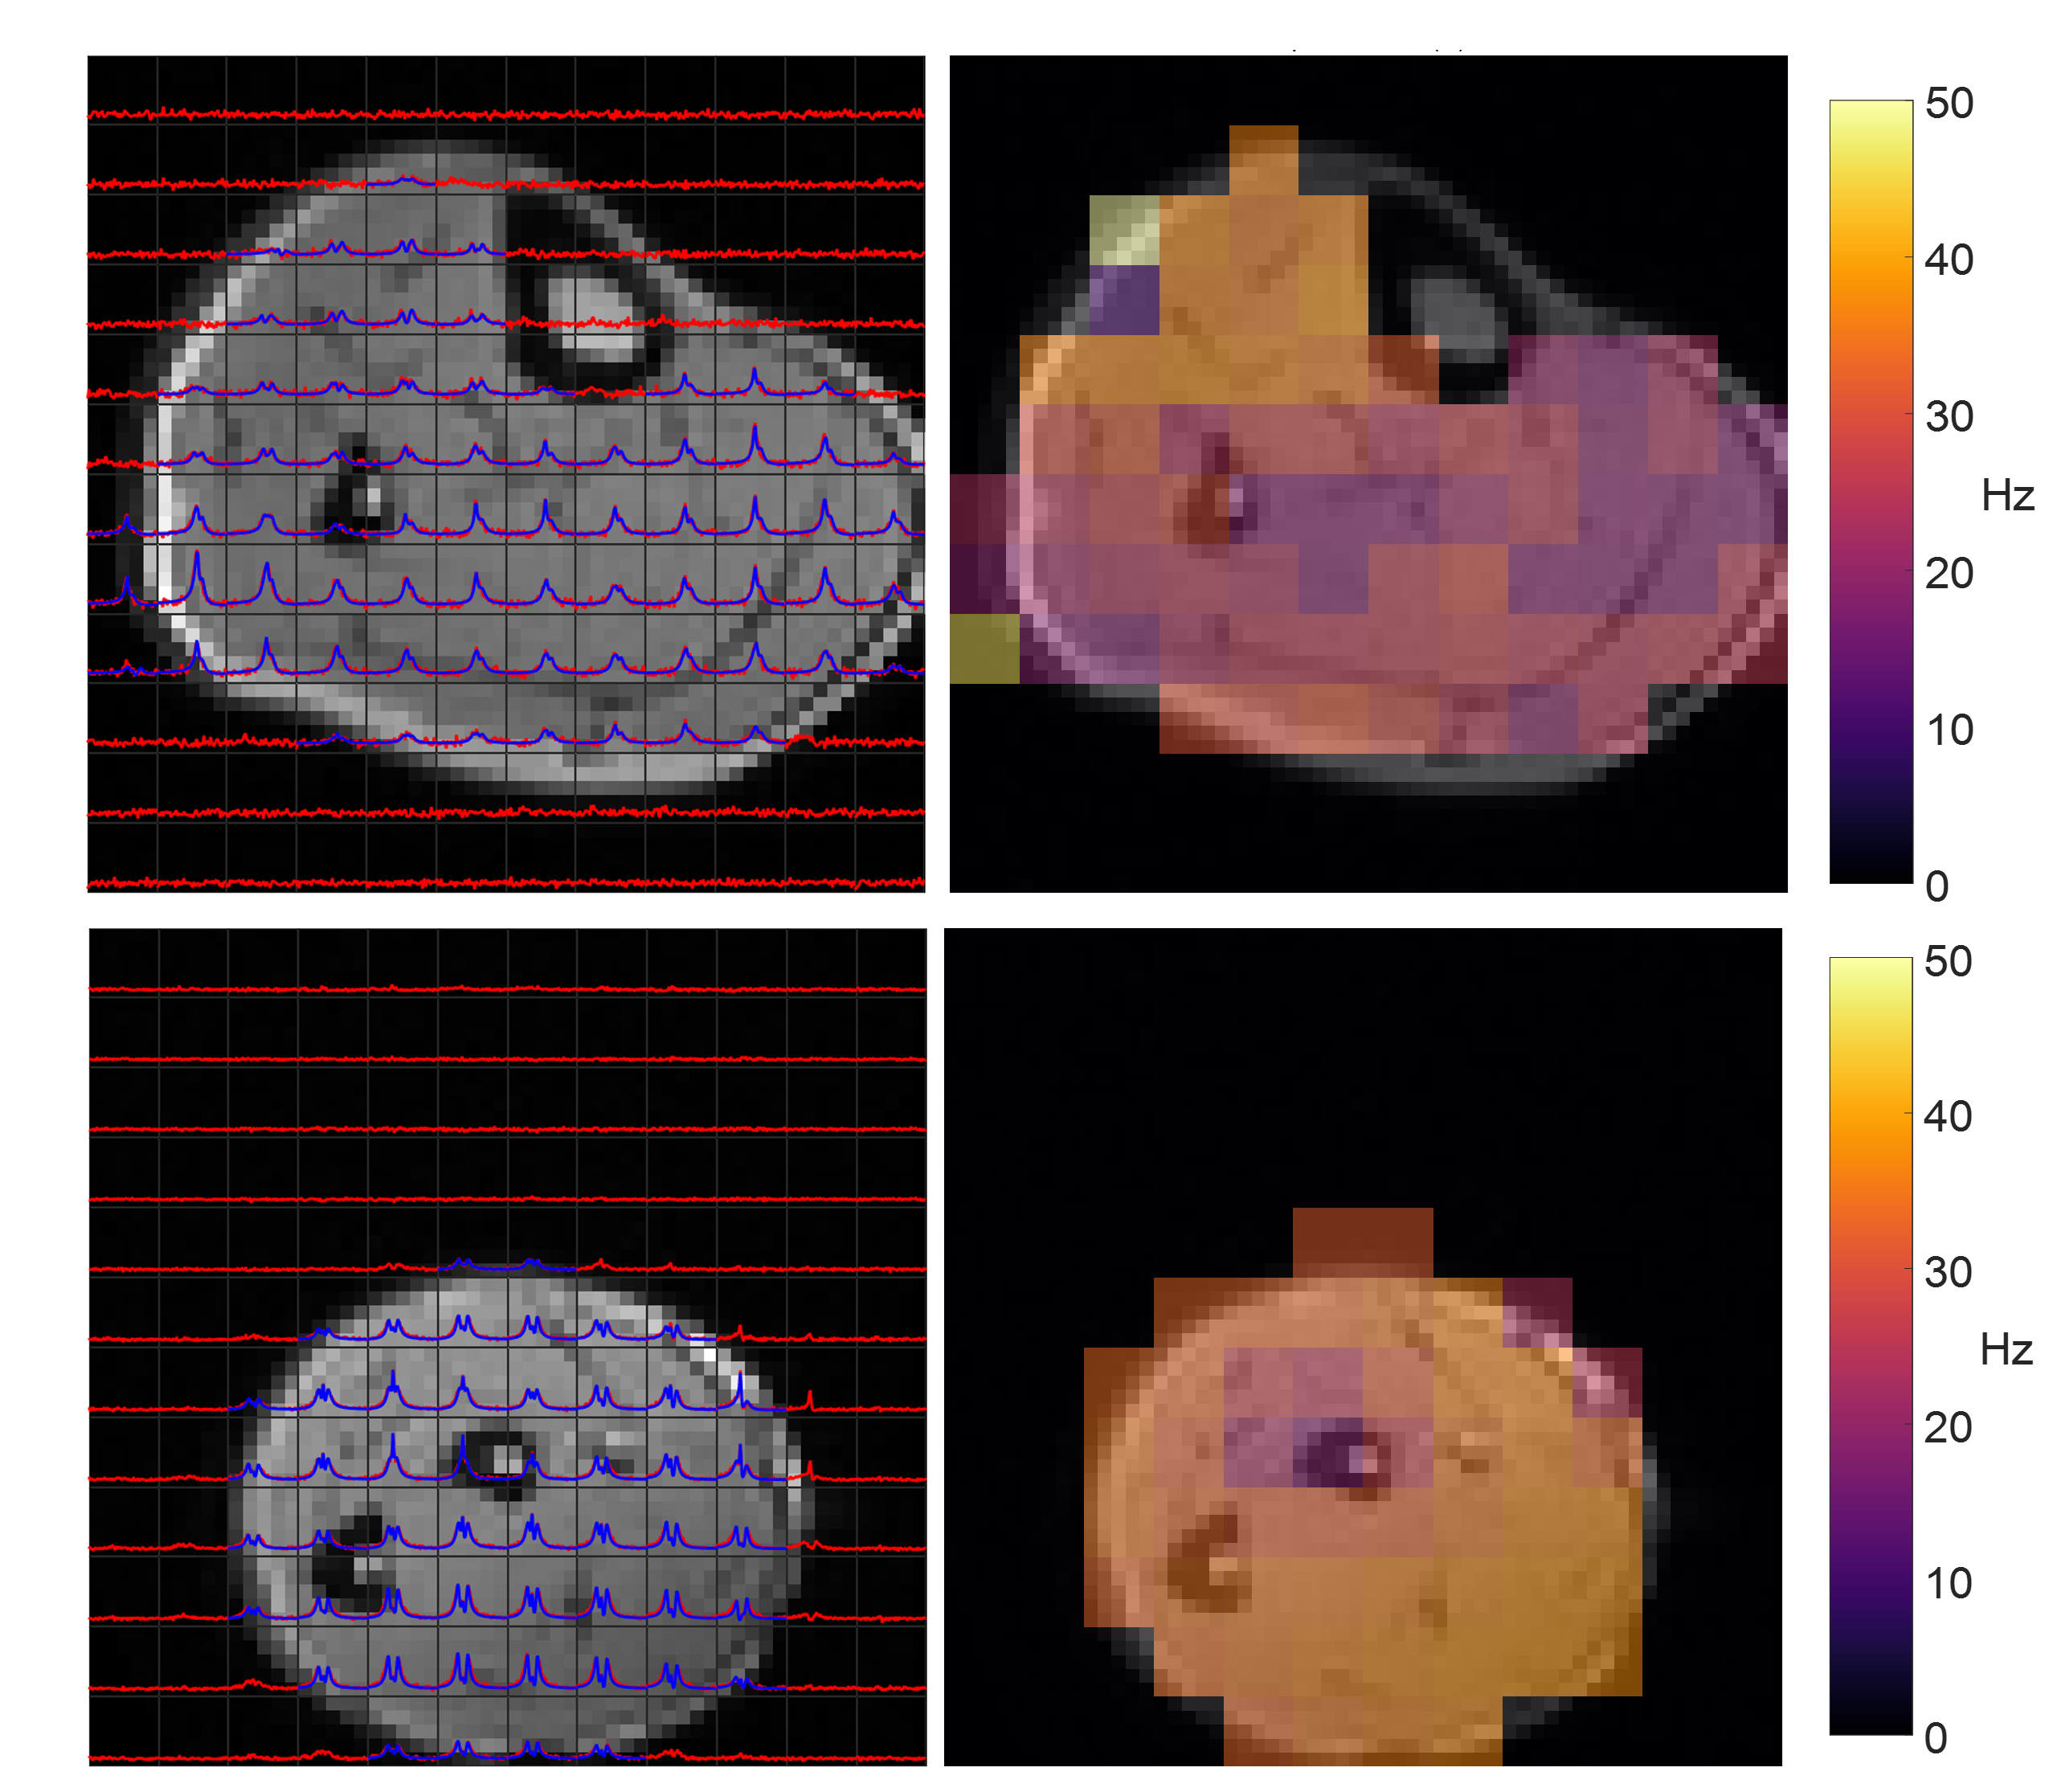
\includegraphics[width=1\textwidth]{Figures/Quad/Calf_Arm_CSI.png}
    \caption{\textit{Example slices from 3D \ac{CSI} of the lower leg (upper panels) and forearm (lower panels), showing spectra (left) and maps of the magnitude of splitting (right). Fits are in blue, CSI data in red. In both cases the limb was approximately aligned with the field.}}
    \label{fig:Quad:Calf_Arm_CSI}
\end{figure}

Figure \ref{fig:Quad:Arm_CSI} shows how the \ac{CSI} spectra from the forearm change as the limb is oriented at different angles to $B_0$. It can be seen that as the forearm gets angled closer to the magic angle (54.74$^\circ$) the quadrupolar splitting vanishes. 

\begin{figure}
    \centering
    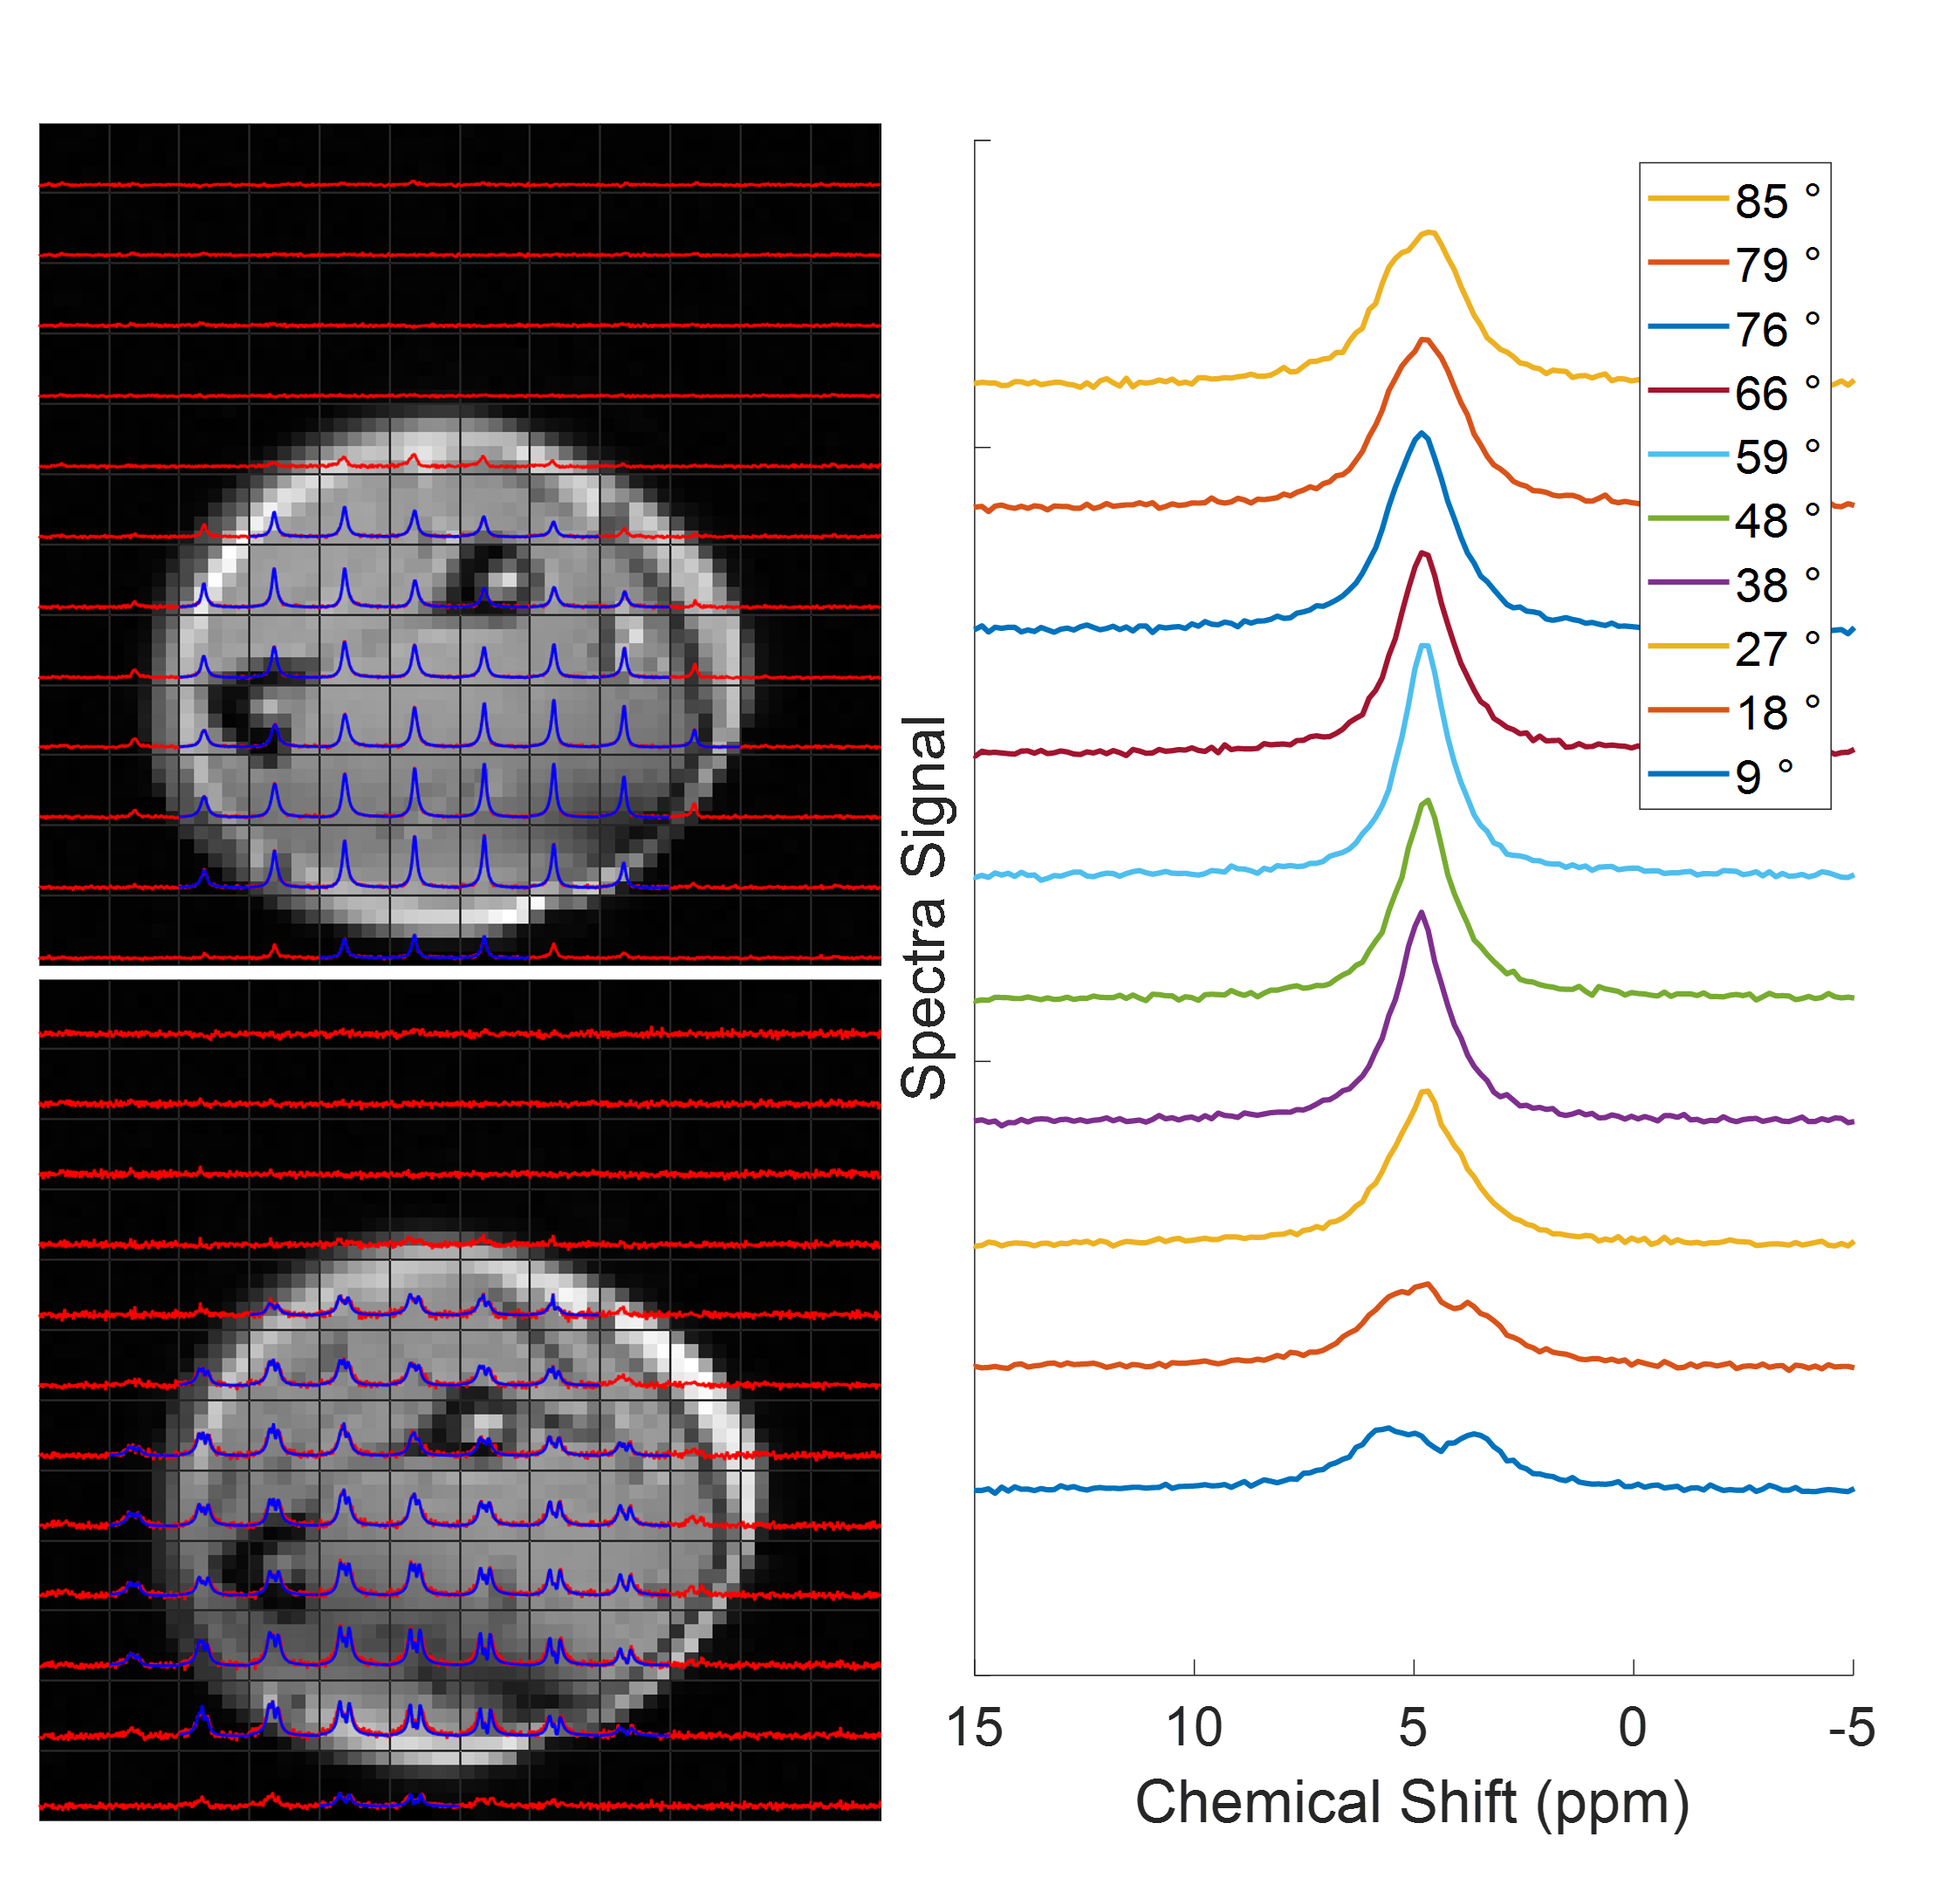
\includegraphics[width=1\textwidth]{Figures/Quad/Arm_CSI_Angle.png}
    \caption{\textit{\ac{CSI} slices of the forearm at two different angles (9$^\circ$, approximately along the field (upper) and 59$^\circ$ (lower), close to the magic angle) to $B_0$ (left panels), with averaged spectra shown for all angles (right panel). Quadrupolar splitting is evident in the 9$^\circ$ \ac{CSI} data, but not seen in the 59$^\circ$ \ac{CSI} data. The average spectra are consistent with quadrupolar splitting that varies with $3\cos^2\theta = 1$ as shown in Eq. \ref{eqn:Quad:Angle}.}}
    \label{fig:Quad:Arm_CSI}
\end{figure}

 Figure \ref{fig:Quad:Split_Angle_2} plots the averaged quadrupolar splitting frequencies against angle. A fit to the expected variation in Eq. \ref{eqn:Quad:Angle} provided an average value for the splitting amplitude across all voxels and participants of 32 $\pm$ 1 Hz. 
 % Which is similar to Figure \ref{fig:Quad:Split_Angle_1} as well as the methodology used to create the Figure except for the improved fitting as well as calculating the angle of the arm using the angle of the bone as oppose as the FOV box. The fit of the splitting frequencies follows the measured splittings better in this case compared to Figure \ref{fig:Quad:Split_Angle_1}.

\begin{figure}
    \centering
    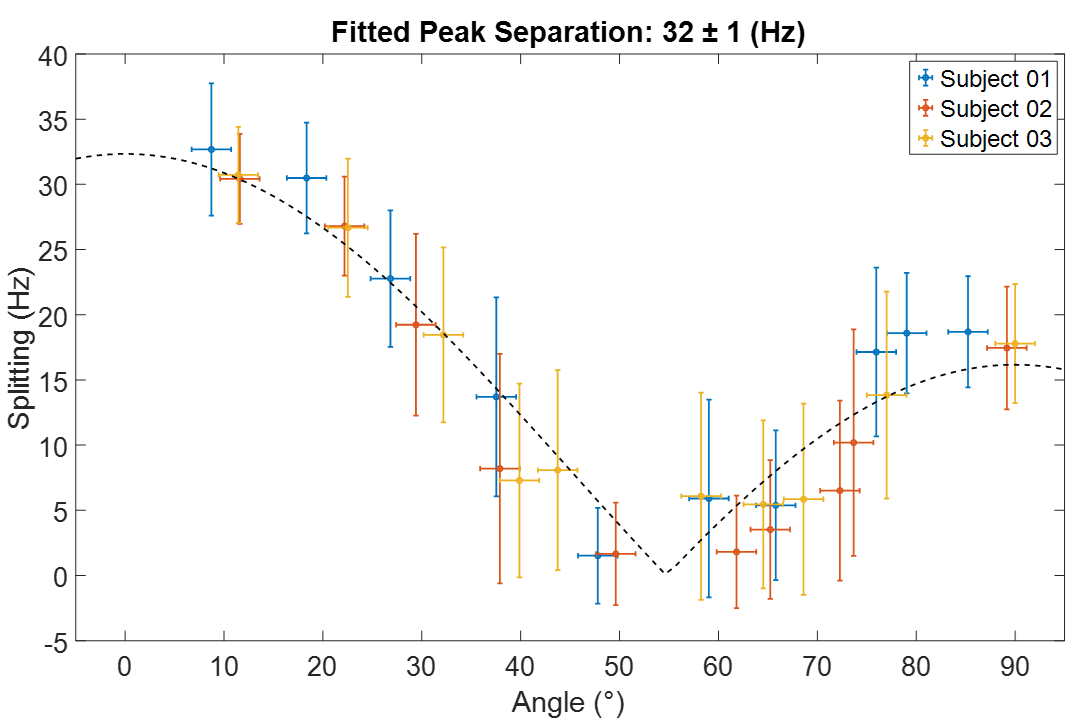
\includegraphics[width=1\textwidth]{Figures/Quad/Split_Angle_2.png}
    \caption{\textit{Average quadrupolar splitting frequencies as a function of forearm angle to $B_0$, fitted to the form of Eq. \ref{eqn:Quad:Amplitude}. Data points are the average splitting over the forearm in each 3D \ac{CSI} data set, with data acquired at 10 different angles from 3 subjects. Error bars show standard deviation of splitting over the volume.}}
    \label{fig:Quad:Split_Angle_2}
\end{figure}

Non-localised \ac{DQF} spectra from the forearm of three participants are plotted as a function of creation time ($\tau$) in Figure \ref{fig:Quad:Bulk_DQF_2}. The biggest differences between participants visible here is the presence of signal at larger $\tau$ values.
% Which is similar to Figure \ref{fig:Quad:Bulk_DQF_1} except more $\tau$ values are used here especially at shorter values. The new fitting method was used here and therefore led to more. The overall behaviour of the forearm spectra here is similar to the forearm spectra in Figure \ref{fig:Quad:Bulk_DQF_1}. accurate fits.

\begin{figure}
    \centering
    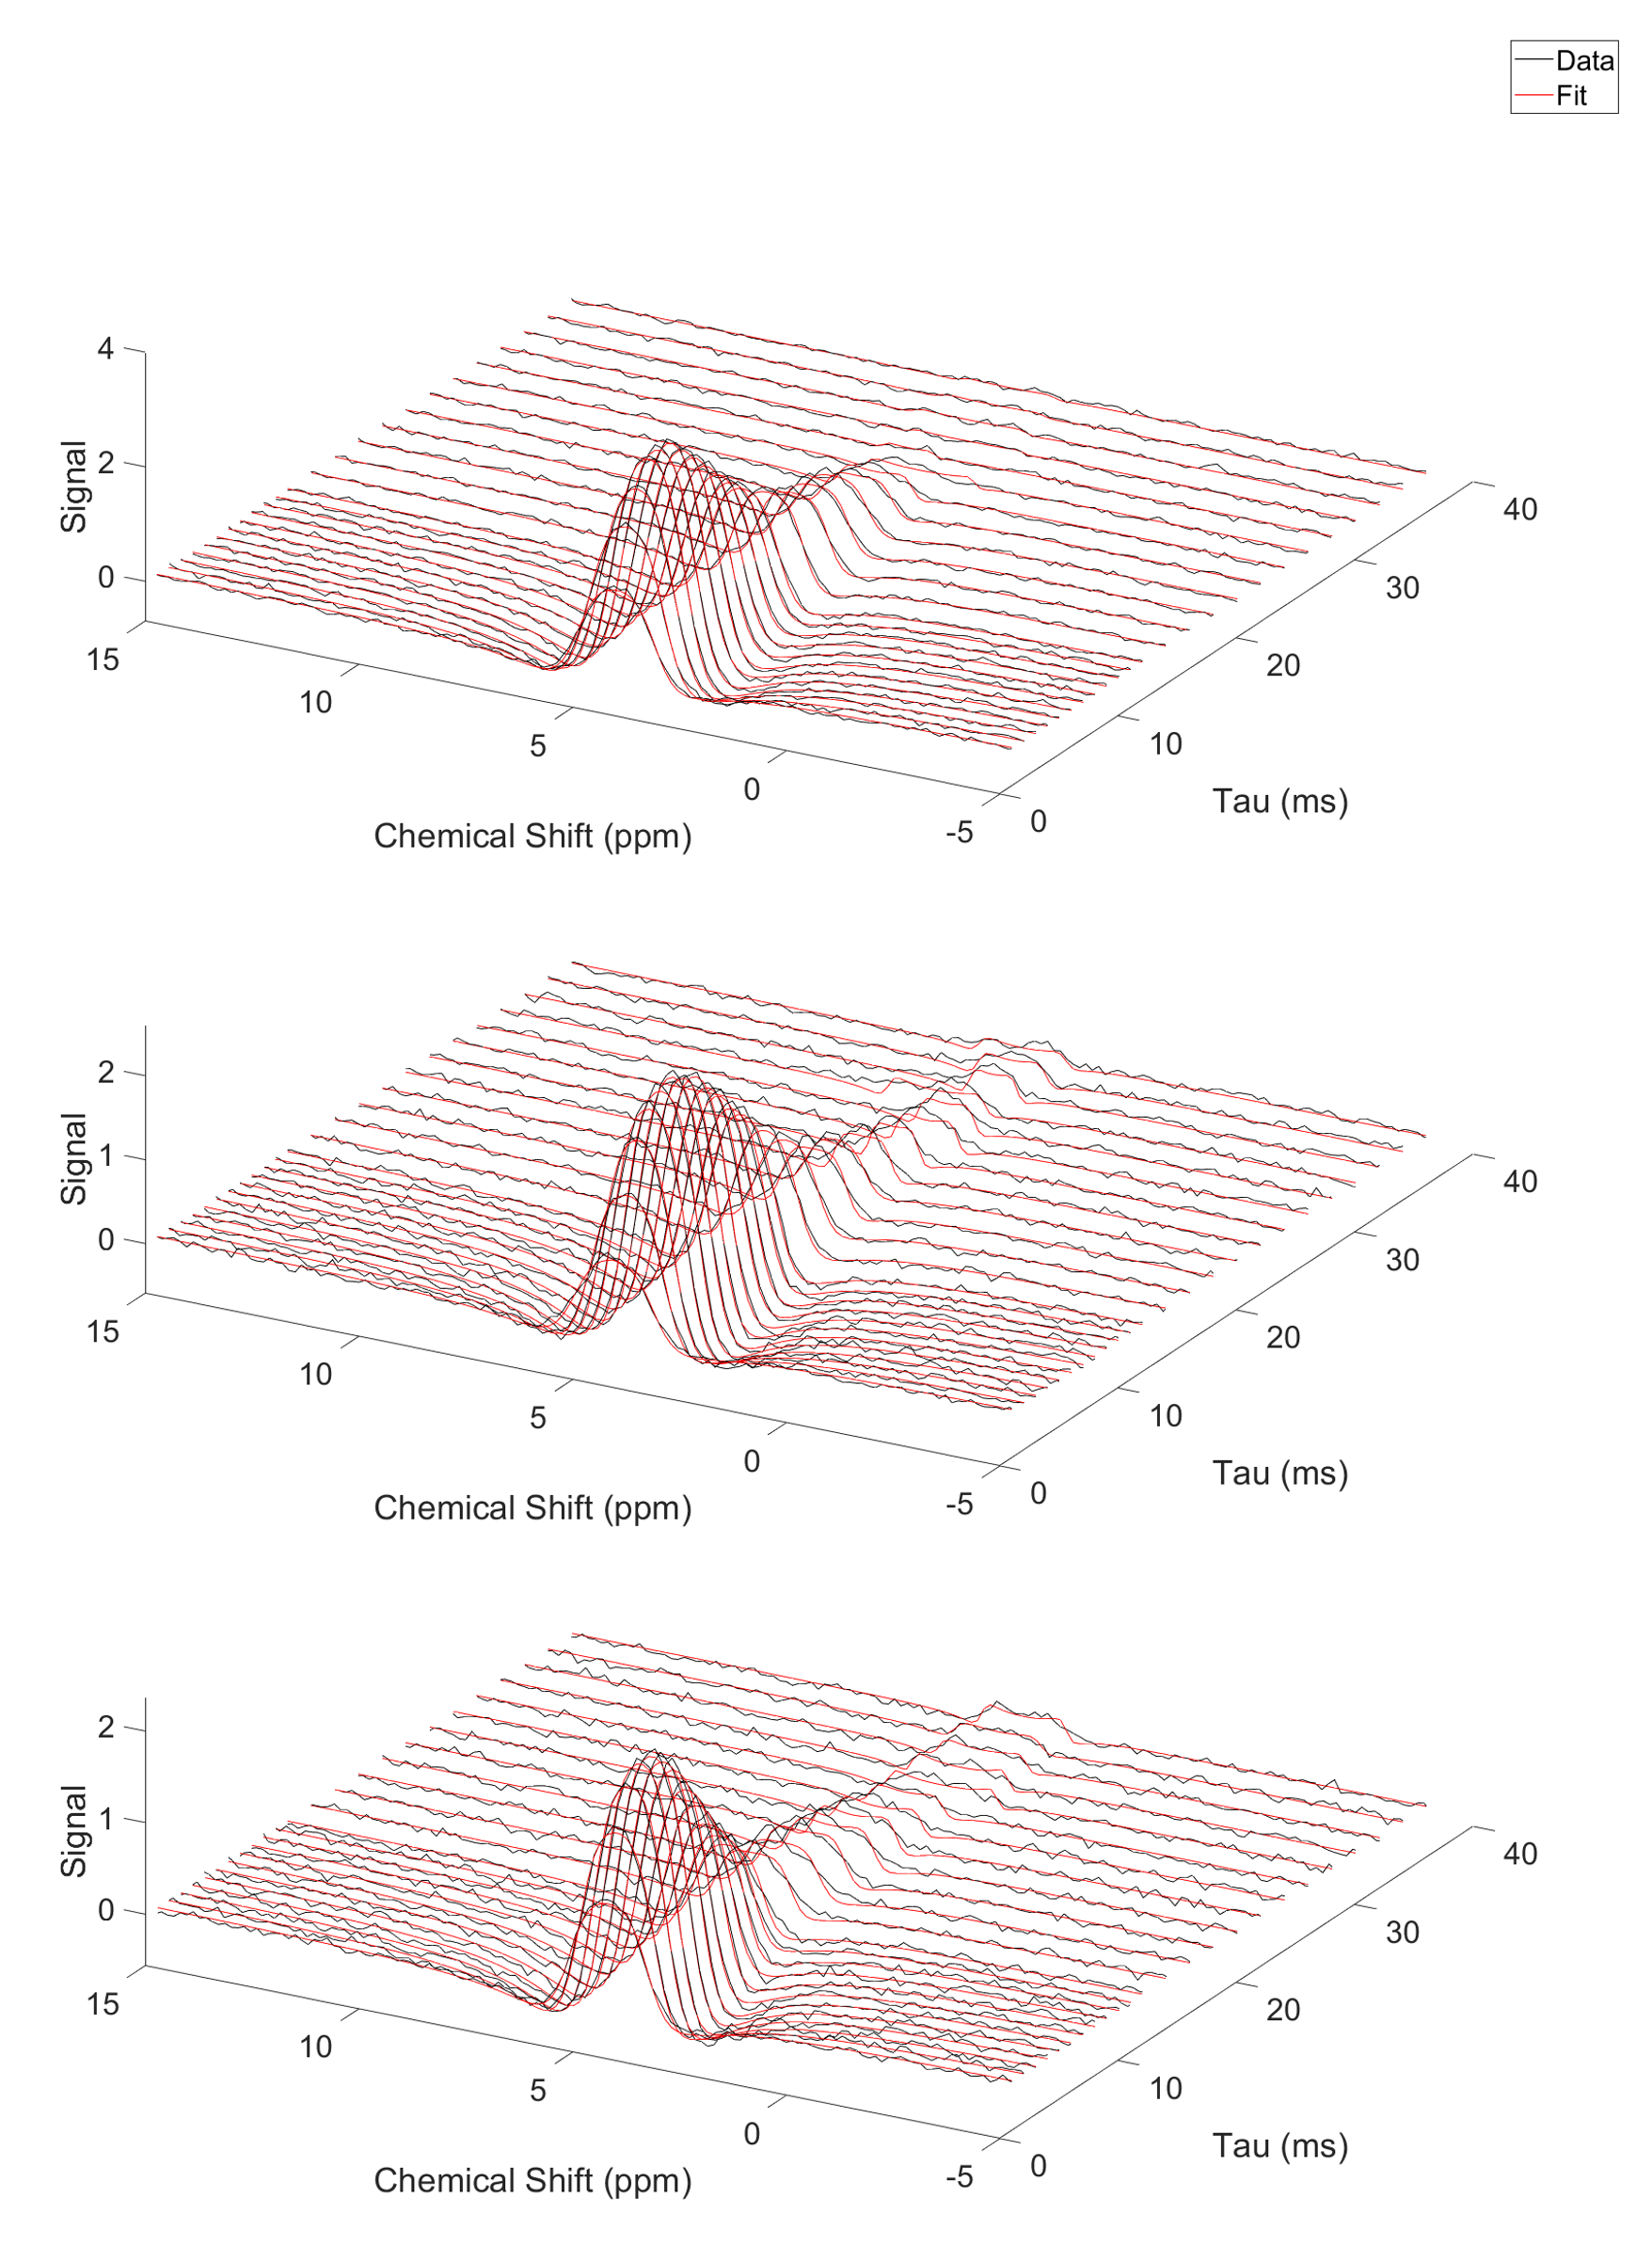
\includegraphics[width=0.8\textwidth]{Figures/Quad/Bulk_DQF_2.png}
    \caption{\textit{\ac{DQF} spectra obtained from a 2 cm axial slice across the forearm (aligned approximately with $B_0$), as a function of the anti-phase \ac{DQF} sequence creation time, $\tau$. Dispersion mode spectra are shown for three subjects, so that the anti-phase doublets produce a symmetric spectrum with maximum amplitude at the centre frequency. The average values of $\nu_q$ found from fitting to these doublets are 36 $\pm$ 7 Hz (top), 31 $\pm$ 5 Hz (middle), and 36 $\pm$ 5 Hz (bottom).}}
    \label{fig:Quad:Bulk_DQF_2}
\end{figure}

Figure \ref{fig:Quad:SQFDQF_2} shows a comparison of 2D pulse-acquire \ac{CSI} and \ac{DQF}-\ac{CSI} data along with fits for the lower leg, highlighting spectra in individual voxels in the \ac{TA} and soleus muscles. 
% This Figure is similar to Figure \ref{fig:Quad:SQFDQF_1} except here the \ac{SNR} is slightly better here thanks to de-noising as well as showing consistent fits to each voxel.

\begin{figure}
    \centering
    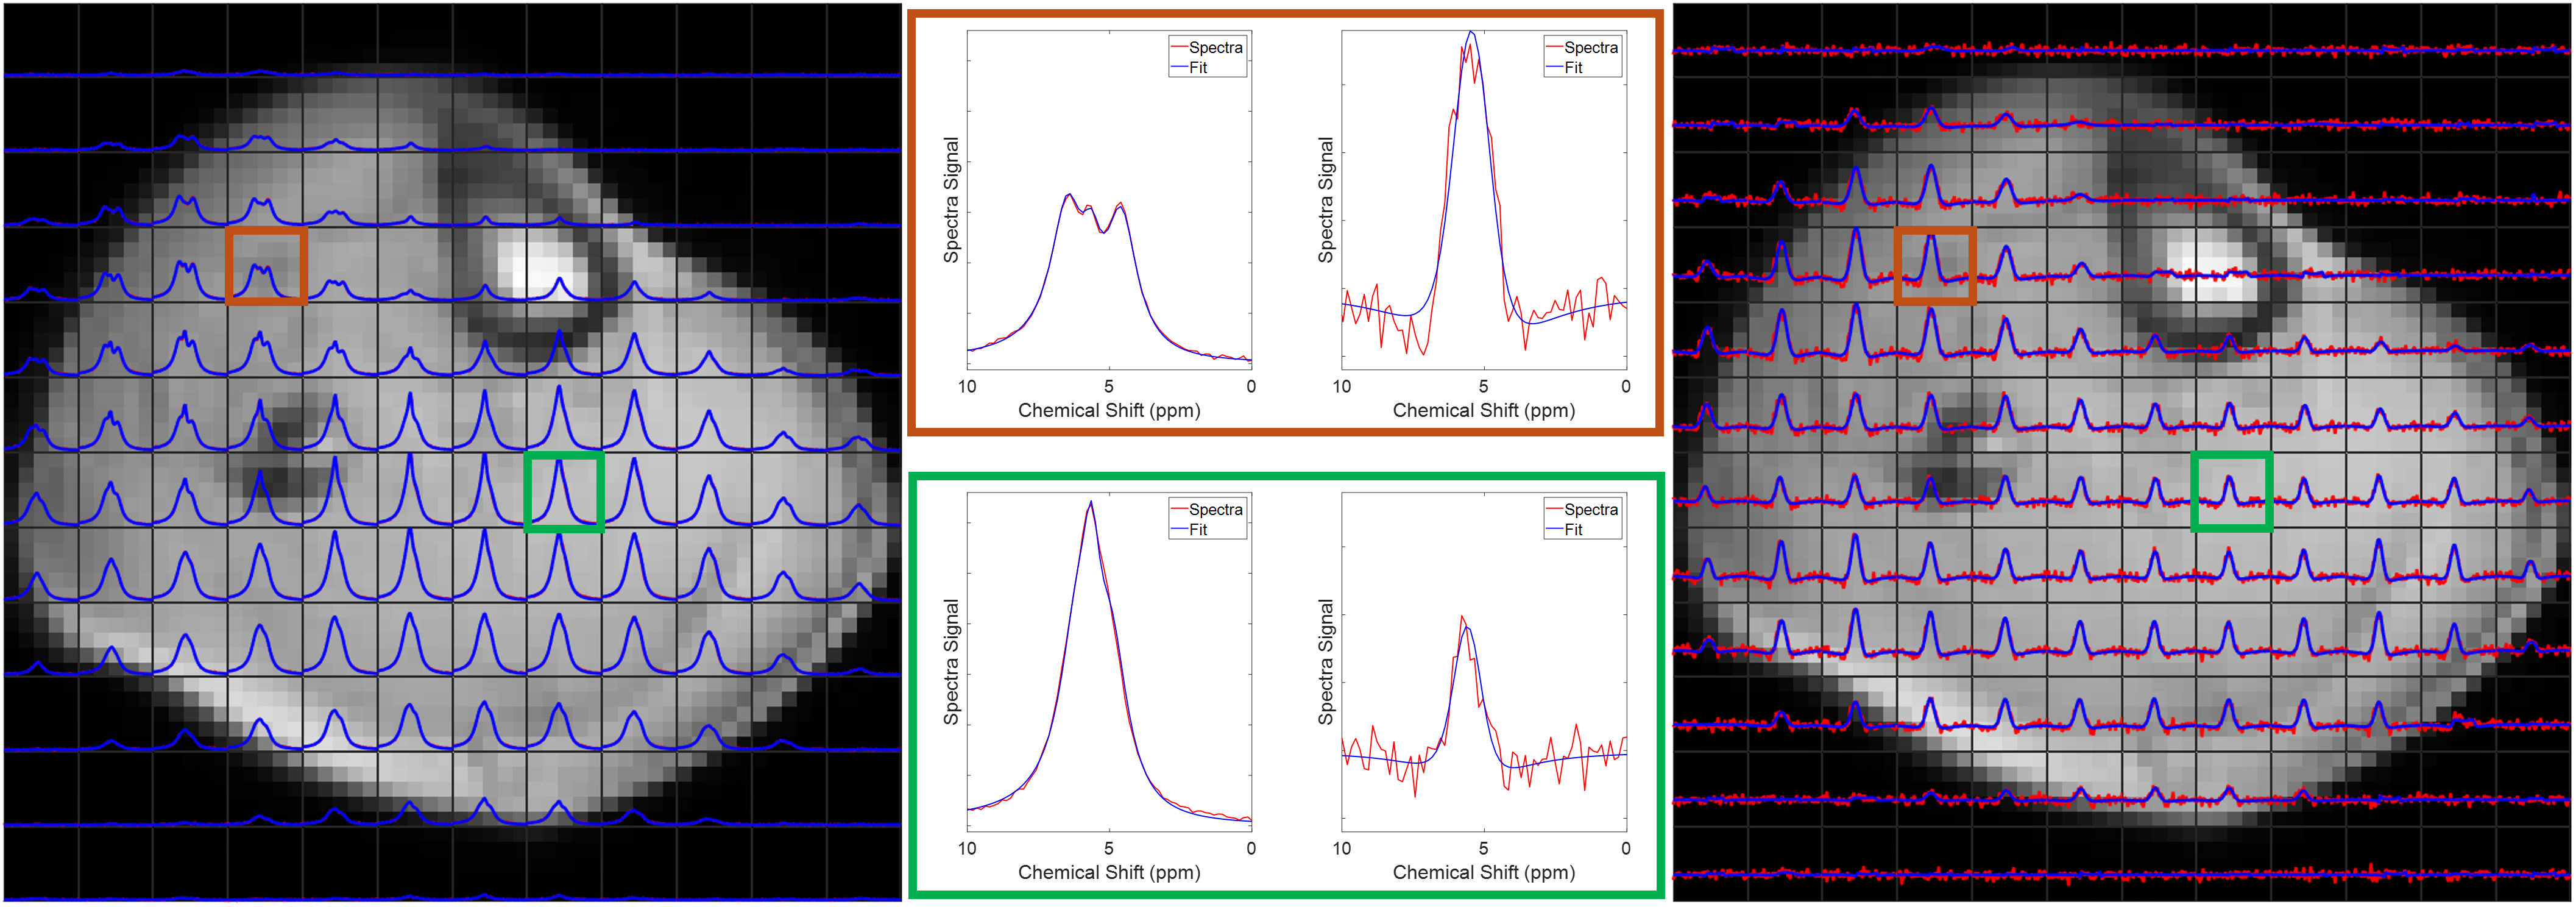
\includegraphics[width=1\textwidth]{Figures/Quad/SQFDQF_CSI_2.png}
    \caption{\textit{Slices of the lower leg from a \ac{CSI} sequence (left) and a \ac{DQF}-\ac{CSI} ($\tau$ = 5 ms) sequence (right), highlighting selected spectra from two voxels: \ac{TA} (orange), soleus (green).}}
    \label{fig:Quad:SQFDQF_2}
\end{figure}

2D \ac{DQF} \ac{CSI} spectra for the lower leg at two different angles, (a) 11$^\circ$ and (b) 65$^\circ$, along with fits are shown in Fig. \ref{fig:Quad:Arm_DQF}. The \ac{SNR} in data acquired at the angle closer to the magic angle is notably smaller compared to the lower angle \ac{CSI}, however fitting was still accurate even in the lower angle data. Also shown are the four voxel \ac{ROI}s that are used for comparison in Fig. \ref{fig:Quad:DQF_CSI_Angle}.

\begin{figure}
    \centering
    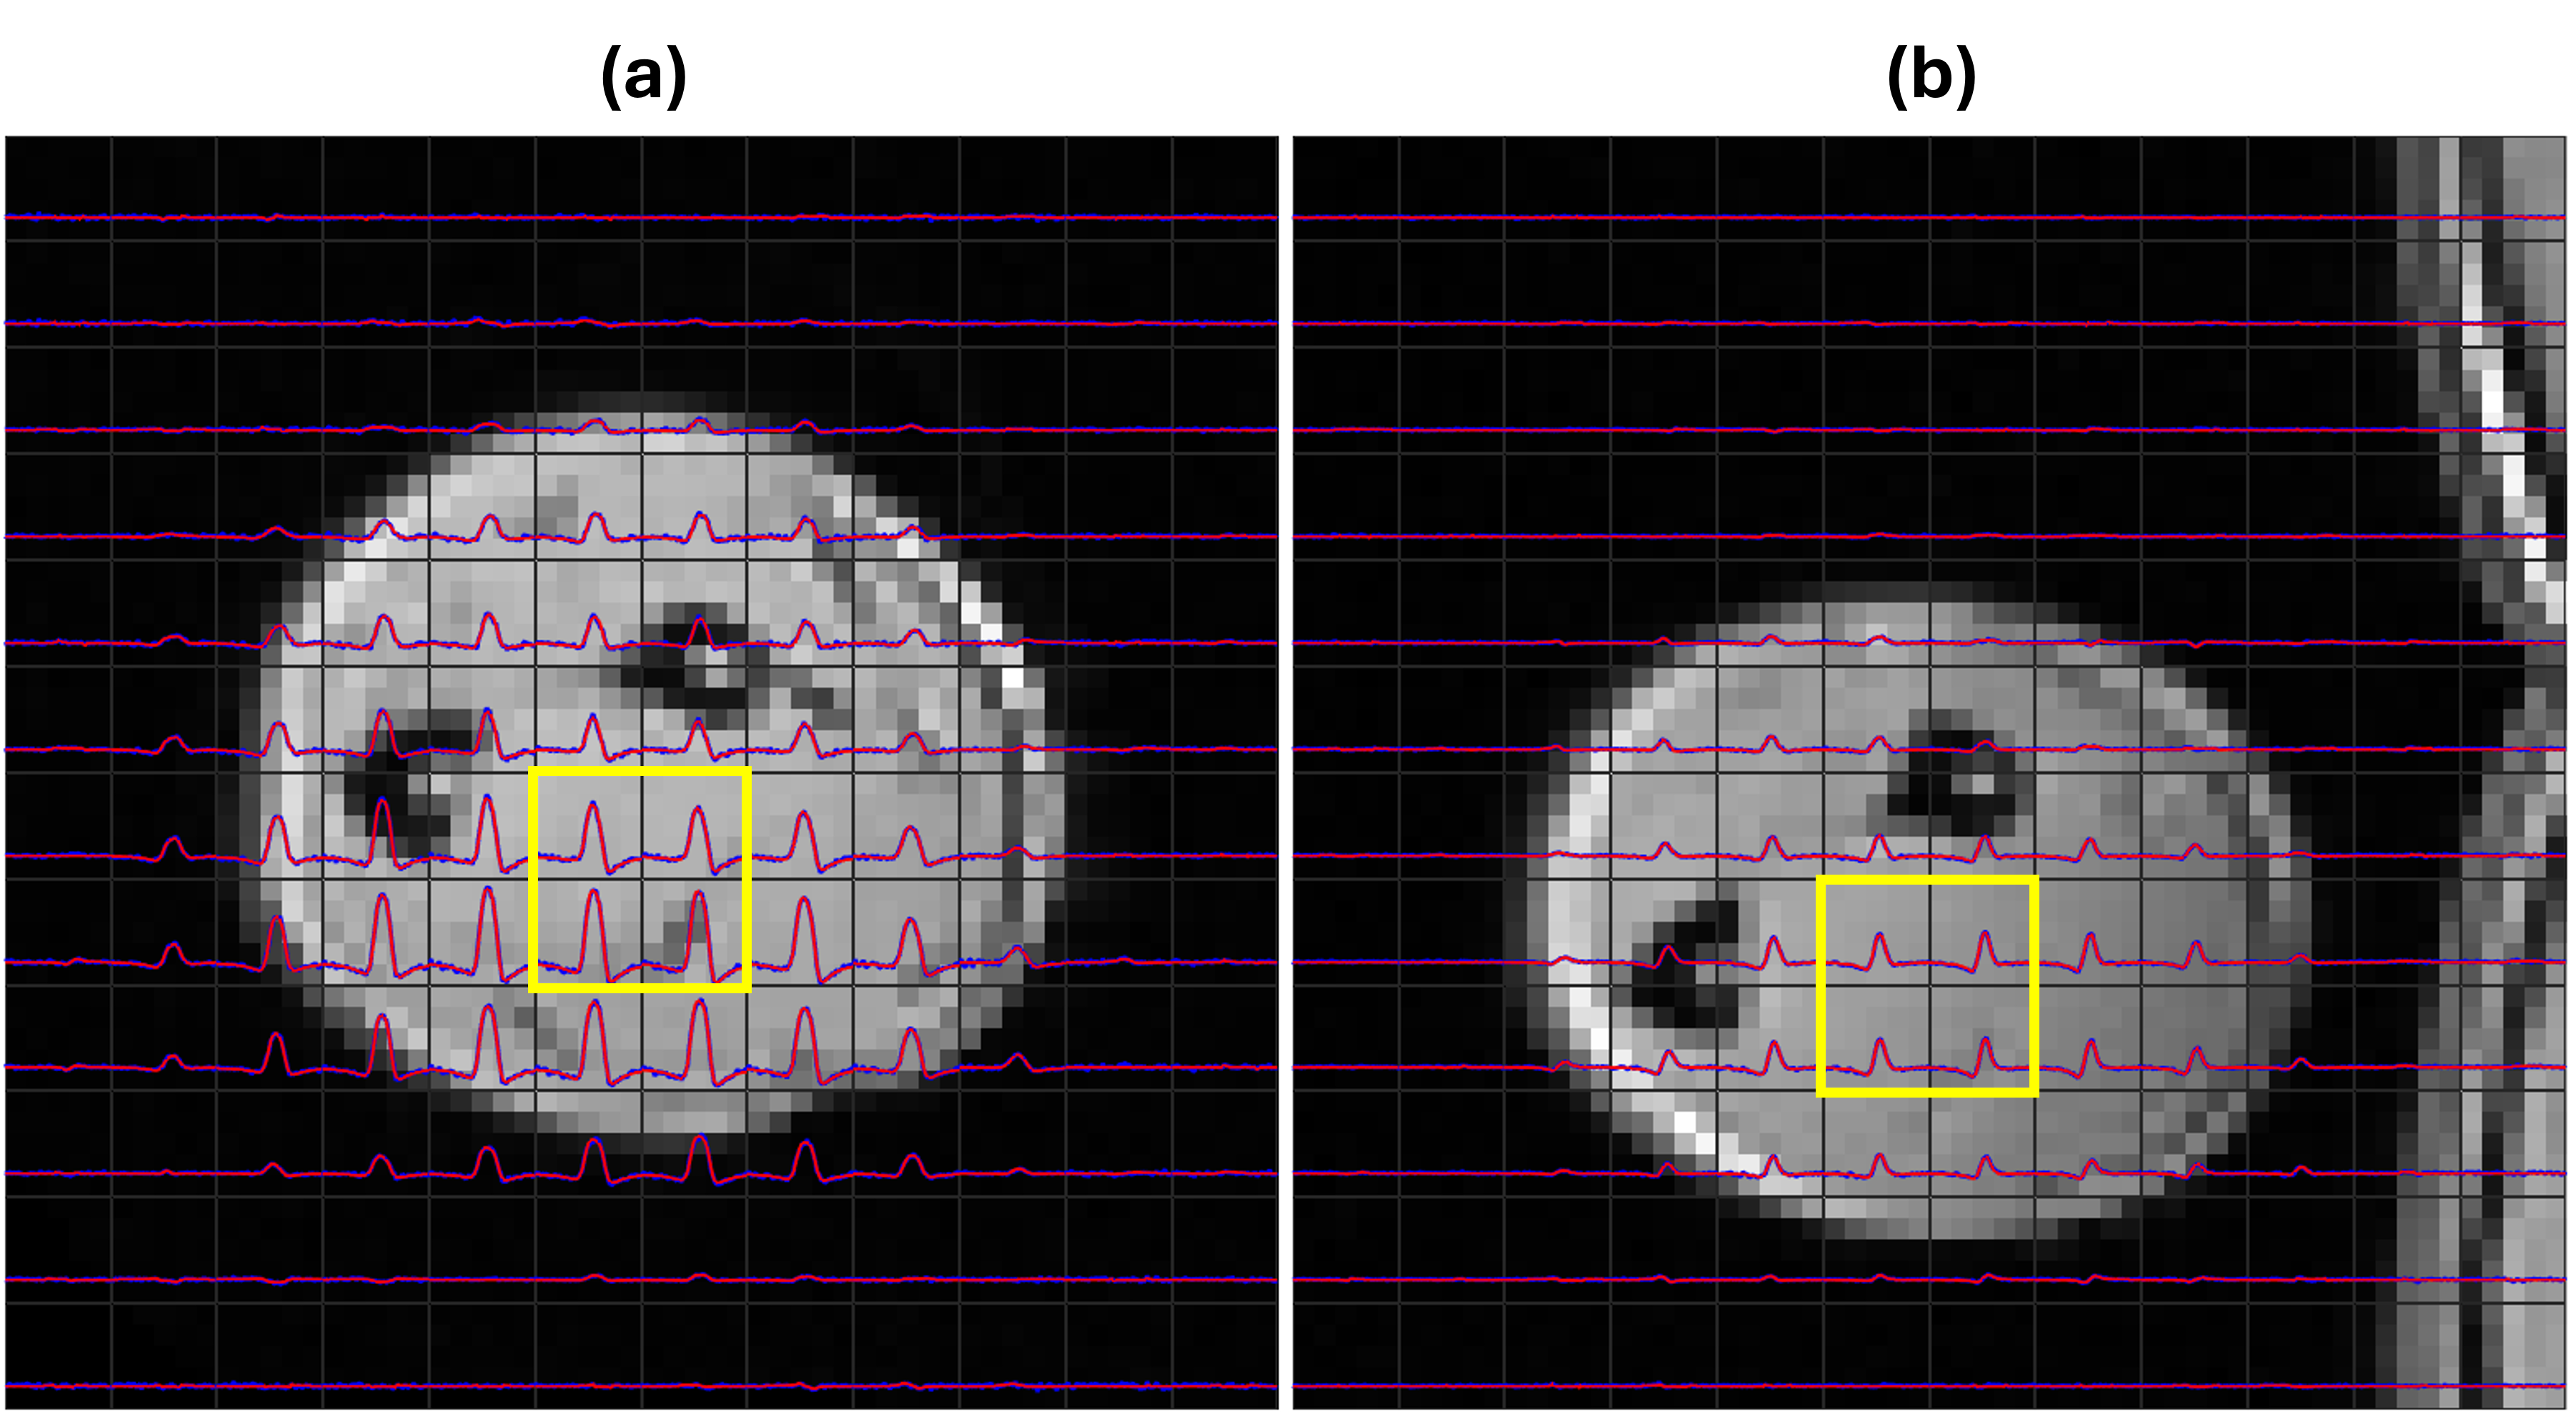
\includegraphics[width=1\textwidth]{Figures/Quad/Arm_DQF.png}
    \caption{\textit{$^2$H 2D \ac{DQF} \ac{CSI} obtained from the same subject's forearm using a Helmholtz coil at two different angles, (a) 11$^\circ$ and (b) 65$^\circ$. The yellow boxes show the \ac{ROI} used to compare spectra in Fig. \ref{fig:Quad:DQF_CSI_Angle}}.}
    \label{fig:Quad:Arm_DQF}
\end{figure}

In Fig. \ref{fig:Quad:DQF_CSI_Angle} a change in \ac{DQF} amplitude is obvious across each subject and across all angles with minimums being in the angle closest to the magic angle which is consistent with equation \ref{eqn:Quad:Amplitude}. The \ac{SNR} is notably lower in subject three's spectra compared to subject's one and two, however still exhibits the same behaviour with fitting still being possible.

\begin{figure}
    \centering
    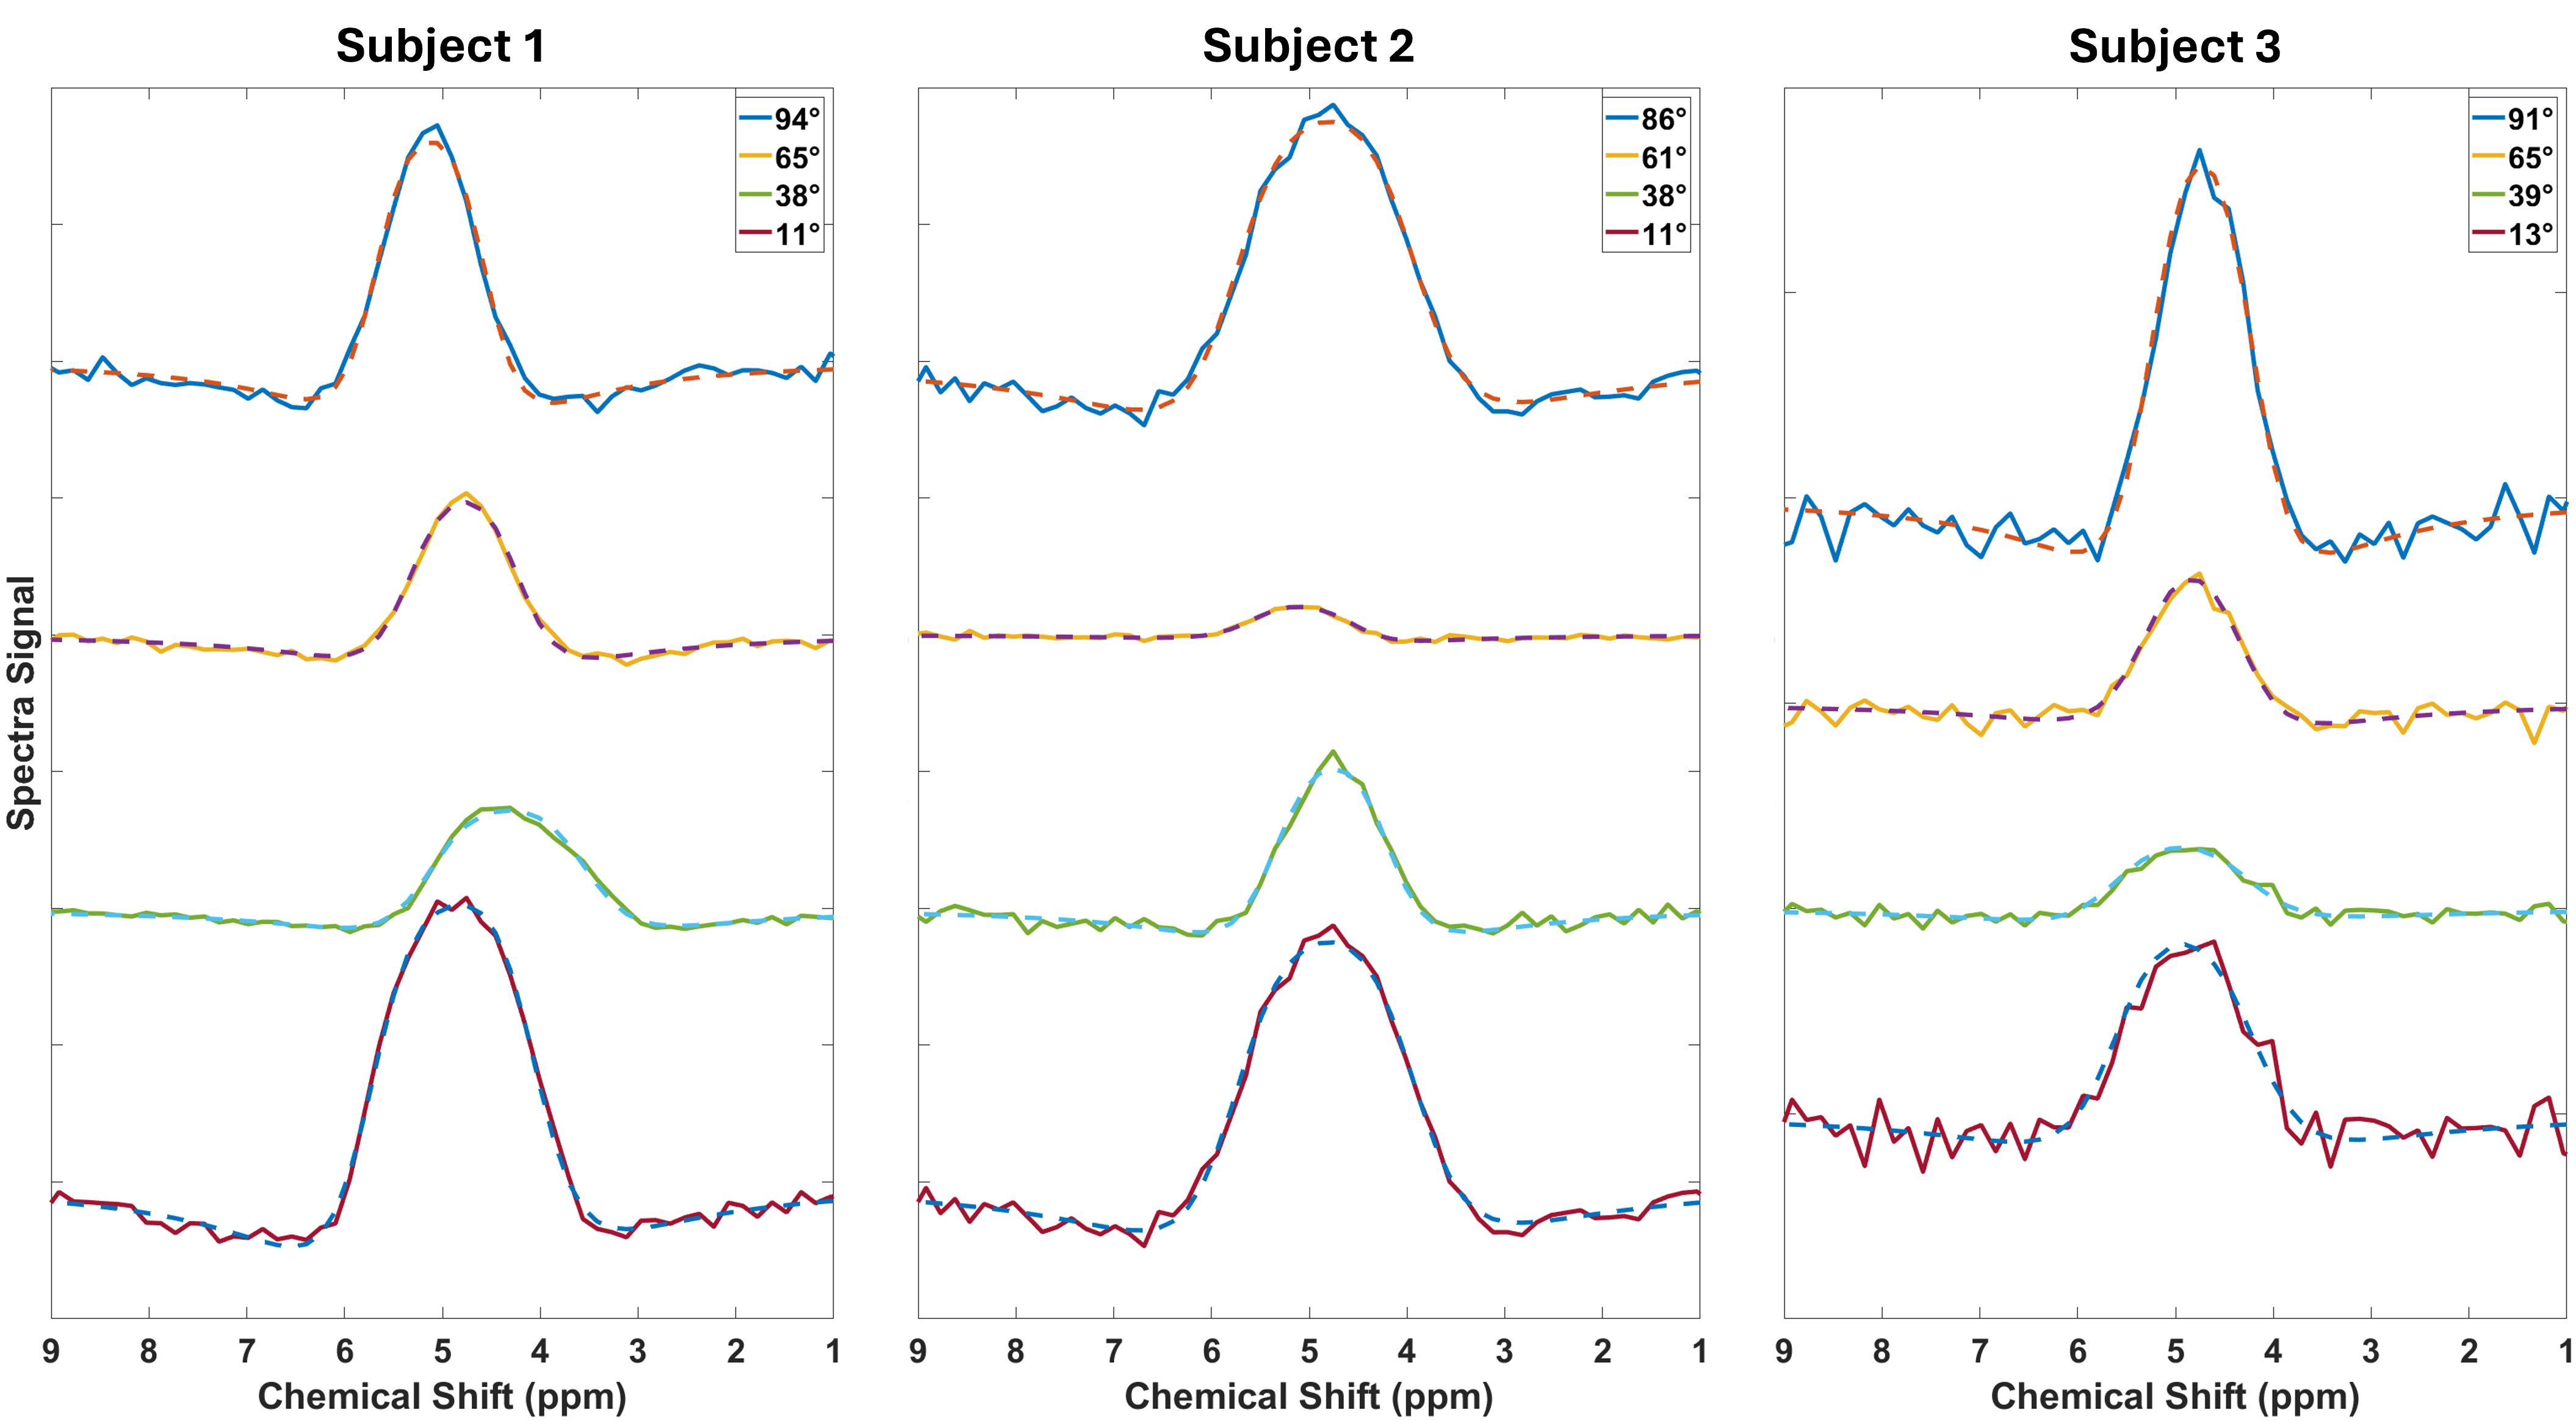
\includegraphics[width=1\textwidth]{Figures/Quad/DQF_CSI_Angle.png}
    \caption{\textit{Four $^2$H spectra averaged together for four angles across three subjects forearms, obtained from \ac{DQF}-\ac{CSI} spectra all stacked on top of each other. Angles relative to the $B_0$ field were measured from the ulna bone.}}
    \label{fig:Quad:DQF_CSI_Angle}
\end{figure}

\section{Discussion}

\subsection{Quadrupolar Splitting}

The residual quadrupolar splitting, seen in figures \ref{fig:Quad:Calf_A}, \ref{fig:Quad:Arm_A} and \ref{fig:Quad:Calf_Arm_CSI}, of the \ac{HDO} spectrum is evidence of local ordering of the tissue and has been previously observed in muscle, tendon, cartilage, and nerves \cite{Gursan2022ResidualMuscle,Sharf1995DetectionNMR-Spectroscopy,Perea20072HDisc,Eliav2016MultipleMRS}. All angular dependencies in this work was performed on the arm due to ease of scanning at multiple specific angles and patient comfort. Other work has performed similar scanning on the lower leg and found magnitude of splittings for different muscle groups which used \ac{NA} $^2$H, higher field strength (7T) at two different angles (0$^\circ$ and 45$^\circ$) \cite{Gursan2022ResidualMuscle}. The splitting map observed in the calf in figures \ref{fig:Quad:Calf_A} and \ref{fig:Quad:Calf_Arm_CSI} is similar to what has been found previously at $\approx$ 0$^\circ$. Because of the spatial splitting in-homogeneity in the lower leg separate \ac{ROI}s for each muscle group had to be used when comparing splitting, this is not as much of a problem in the arm (as can be seen in figures \ref{fig:Quad:Calf_A} and \ref{fig:Quad:Calf_Arm_CSI}) which is why only a single  ROI is used here. The largest separation arises in the TA muscle group which can be due to the fibres of this muscle align closely \cite{Gursan2022ResidualMuscle} with the $B_0$-direction, but it could also indicate a more ordered environment in which the water resides. Separate \ac{ROI} analysis here in the main three forearm muscle groups (mobile wad, dorsal and volar compartments) would have been interesting to see if any small difference was present. However, due to the large voxels and low \ac{SNR} from using the built-in body coil for the anatomical images. 

Initially MATLAB's fmincon function was used to determine the minimum of the sum of the residuals squared between two/three Lorentzian peaks and the experimental data. Whichever number of peaks that provided the lower minimum value was used for the fitting. In a purely anisotropic medium where the entire signal has been separated into a doublet through quadrupolar splittings a two-peak Lorentzian would accurately model the data. Due to the low spatial resolution of the \ac{CSI} scans realistically there is a combination of separated doublets and single peaks present which is represented by a three-peak fit. A three-peak fit could be used to fit all voxels as long as each peak is fully resolved, this is often the case here as the linewidth is often larger than the separation. Therefore, in some cases a three-peak fit would result in misaligned fitting which is why this swap in choice of number of peaks was used. The OXSA-AMARES MATLAB toolbox has already been shown to improve fitting over other methods by the increase in the number of prior knowledge. This has lead to increase reliability in fitting here which allows the use of more consistent three-peak fitting in the time domain. The change in fitting routine hasn't changed the overall spatial trend in the maps of the separation frequencies, which can be seen in Figure \ref{fig:Quad:Calf_A} and \ref{fig:Quad:Calf_Arm_CSI}.

It is difficult to say whether the change in fitting, the de-noising  or the change in angle determination (\ac{FOV} box angle or the angle of the ulna) or even the extra subjects dataset has primarily led to the increase in fitting to equation \ref{eqn:Quad:Angle} in Figure \ref{fig:Quad:Split_Angle_2} compared to Figure \ref{fig:Quad:Split_Angle_1}. However, since the angle of the ulna can be significantly different to the angle of the \ac{FOV} box, it is suspected that this is the driving force for the increase in fitting accuracy. With that being said the use of all these changes is important.

\subsection{DQF}

As is seen with the \ac{DQF} filtered \ac{CSI} data it can be difficult to identify where the regions of maximum \ac{DQF} signal are present due to the lack of spectral resolve in the anti-phase peaks. However, in figures \ref{fig:Quad:SQFDQF_1} and \ref{fig:Quad:SQFDQF_2} an increase in the \ac{TA} and gastrocnemius msucle and a decrease in the soleus muscle is visible which is consistent with separations from pulse-acquire \ac{SQF} results in figures \ref{fig:Quad:Calf_A} and \ref{fig:Quad:Calf_Arm_CSI}. Whilst \ac{DQF} scans have the ability to suppress \ac{SQF} signals, the \ac{DQF} signal depends on how ordered is a tissue. Therefore, analysing a creation-time ($\tau$) non-localised \ac{DQF} series could be more complicated as could contain multiple splitting frequencies ($\nu_q$) and T$_2$ times in equation \ref{eqn:Quad:Amplitude}. This is why the behaviour between the forearm and lower leg spectra and amplitude variations differ so much in figures \ref{fig:Quad:Bulk_DQF_1} and \ref{fig:Quad:BuildUp}. And whilst fittings are plotted in Figure \ref{fig:Quad:BuildUp} it is clear this model does not suit the data very well, this could be due to resonance offsets, flip angle errors and potentially a range of quadrupolar frequencies \cite{Sharf1995DetectionNMR-Spectroscopy} (as has already been pointed out. 

Fits to eight \ac{DQF} datasets from study one (which included the datasets in Figure \ref{fig:Quad:Bulk_DQF_1}) produced a mean and standard deviation of $\nu_q$ = 39.7 $\pm$ 11.5 Hz. However, in all curves, a global maximum is seen at approximately 2$\tau \approx$ 15 ms, which would correspond to approximately $\nu_q \approx$ 33 Hz. As a comparison, mean values obtained by fitting all \ac{DQF} spectra in each dataset produced $\nu_q$ = 29.5 $\pm$ 3.7 Hz, which is in closer agreement with values similarly measured in the lower leg \cite{Gursan2022ResidualMuscle}. 

By using more $\tau$ values in Figure \ref{fig:Quad:Bulk_DQF_2} in a similar range than what we used previously in Figure \ref{fig:Quad:Bulk_DQF_1}, a more complete evolution of the \ac{DQF} signal in the forearm is possible. Whilst still having the similar characteristics to the forearm curves in Figure \ref{fig:Quad:BuildUp}, the repeated forearm curves in Figure \ref{fig:Quad:Bulk_DQF_2} have a slower evolution and are more similar to the calf curves. By using OXSA-AMARES \cite{Purvis2017OXSA:MATLAB} more reliable and accurate fitting are possible even at larger $\tau$ values with lower SNR. From having a more complete model extra features are visible in the amplitude changes in Figure \ref{fig:Quad:Bulk_DQF_2}, such as extra signal such that its not an exponential decay as is shown in equation \ref{eqn:Quad:Amplitude}. This extra signal is due to the same reasons as why Figure \ref{fig:Quad:BuildUp} doesn't follow the model very well, poor flip angles, off resonance effects and contributions from multiple splitting frequencies \cite{Sharf1995DetectionNMR-Spectroscopy}. the effect from multiple splitting frequencies was aimed to be decreased by using the arm as oppose to the lower leg. The data in Figure \ref{fig:Quad:Bulk_DQF_2} hasn't been modelled as it is clear a more complicated model is needed, which involves off resonance and flip angle effects.

Whilst the buildup couldn't be correctly modelled the angular response of \ac{DQF} signal has been explored in Figure \ref{fig:Quad:DQF_CSI_Angle}. A full response curve similar to Figure \ref{fig:Quad:Split_Angle_2} was not possible as only four angles have been measured. However, it is enough to see that the data approximately follows equation \ref{eqn:Quad:Angle} with minimum signal around the magic angle (54.74$^\circ$) and maximum with a straight arm (0$^\circ$ to the $B_0$ field).

\subsection{Future and Limitations}

These are the first results using $^2$H for \textit{in vivo} \ac{DQF} spectroscopy, and as such there are areas for improvement and developing the technique further. By using dual-tuned coils it is possible to not only acquire $^2$H data as well as high resolution anatomical $^1$H images, which would allow improved segmentation and \ac{ROI} analysis. In this case it would allow specific muscle group separation and \ac{DQF} signals to be identified. An improved \ac{RF} coil with multiple channels for the $^2$H would also increase \ac{SNR} which would allow for better spatial resolution and reduce effect from multiple quadrupolar separations.

On the topic of hardware \ac{RF} coil improvements, if the $B_0$ field strength is increased say from 3T to 7T this would improve the spectral resolution. More well resolved peaks means that fitting will be improved and scan time could potentially be reduced to allow for more dynamic scanning.

Whilst the \ac{HDO} \ac{DQF} peaks overlap which creates one strong central signal, a \ac{DQF} imaging sequence could be used instead of a spectroscopic sequence. This would reduce scan time which could allow for more averaging to improve \ac{SNR}, improve spatial resolution on \ac{CSI} acquisitions or acquire more dynamic data ie. with more angles or more $\tau$ values.

\section{Conclusion}

Here the first \textit{in vivo} $^2$H \ac{DQF} datasets have been shown which would allow crucial information on the ordering of local tissue. This has been performed at clinical field strength which shows that in the future (with more improvements to study protocol) this technique could be used as a diagnostic tool, for diseases that have so far only been shown on \textit{ex vivo} data \cite{Ooms2015DoubleTissue, Sharf1995DetectionNMR-Spectroscopy, Perea20072HDisc, Sun2010InvestigationNMR}. The quadrupolar seperation has also been quantified in different muscle groups in the lower leg and in the calf as a whole, as well as the angular dependence on this behaviour. By improving the \ac{RF} coil used, increasing the field strength and using imaging sequences this technique shows real promise in uncovering useful information of tissue ordering.

% \printbibliography % Comment out main doc

% \end{document}